% Options for packages loaded elsewhere
% Options for packages loaded elsewhere
\PassOptionsToPackage{unicode}{hyperref}
\PassOptionsToPackage{hyphens}{url}
\PassOptionsToPackage{dvipsnames,svgnames,x11names}{xcolor}
%
\documentclass[
  12pt,
  oneside]{book}
\usepackage{xcolor}
\usepackage[top=30mm,bottom=30mm,left=25mm,right=20mm,headheight=15mm,footskip=33pt]{geometry}
\usepackage{amsmath,amssymb}
\setcounter{secnumdepth}{5}
\usepackage{iftex}
\ifPDFTeX
  \usepackage[T1]{fontenc}
  \usepackage[utf8]{inputenc}
  \usepackage{textcomp} % provide euro and other symbols
\else % if luatex or xetex
  \usepackage{unicode-math} % this also loads fontspec
  \defaultfontfeatures{Scale=MatchLowercase}
  \defaultfontfeatures[\rmfamily]{Ligatures=TeX,Scale=1}
\fi
\usepackage{lmodern}
\ifPDFTeX\else
  % xetex/luatex font selection
\fi
% Use upquote if available, for straight quotes in verbatim environments
\IfFileExists{upquote.sty}{\usepackage{upquote}}{}
\IfFileExists{microtype.sty}{% use microtype if available
  \usepackage[]{microtype}
  \UseMicrotypeSet[protrusion]{basicmath} % disable protrusion for tt fonts
}{}
\usepackage{setspace}
\makeatletter
\@ifundefined{KOMAClassName}{% if non-KOMA class
  \IfFileExists{parskip.sty}{%
    \usepackage{parskip}
  }{% else
    \setlength{\parindent}{0pt}
    \setlength{\parskip}{6pt plus 2pt minus 1pt}}
}{% if KOMA class
  \KOMAoptions{parskip=half}}
\makeatother
% Make \paragraph and \subparagraph free-standing
\makeatletter
\ifx\paragraph\undefined\else
  \let\oldparagraph\paragraph
  \renewcommand{\paragraph}{
    \@ifstar
      \xxxParagraphStar
      \xxxParagraphNoStar
  }
  \newcommand{\xxxParagraphStar}[1]{\oldparagraph*{#1}\mbox{}}
  \newcommand{\xxxParagraphNoStar}[1]{\oldparagraph{#1}\mbox{}}
\fi
\ifx\subparagraph\undefined\else
  \let\oldsubparagraph\subparagraph
  \renewcommand{\subparagraph}{
    \@ifstar
      \xxxSubParagraphStar
      \xxxSubParagraphNoStar
  }
  \newcommand{\xxxSubParagraphStar}[1]{\oldsubparagraph*{#1}\mbox{}}
  \newcommand{\xxxSubParagraphNoStar}[1]{\oldsubparagraph{#1}\mbox{}}
\fi
\makeatother


\usepackage{longtable,booktabs,array}
\newcounter{none} % for unnumbered tables
\usepackage{calc} % for calculating minipage widths
% Correct order of tables after \paragraph or \subparagraph
\usepackage{etoolbox}
\makeatletter
\patchcmd\longtable{\par}{\if@noskipsec\mbox{}\fi\par}{}{}
\makeatother
% Allow footnotes in longtable head/foot
\IfFileExists{footnotehyper.sty}{\usepackage{footnotehyper}}{\usepackage{footnote}}
\makesavenoteenv{longtable}
\usepackage{graphicx}
\makeatletter
\newsavebox\pandoc@box
\newcommand*\pandocbounded[1]{% scales image to fit in text height/width
  \sbox\pandoc@box{#1}%
  \Gscale@div\@tempa{\textheight}{\dimexpr\ht\pandoc@box+\dp\pandoc@box\relax}%
  \Gscale@div\@tempb{\linewidth}{\wd\pandoc@box}%
  \ifdim\@tempb\p@<\@tempa\p@\let\@tempa\@tempb\fi% select the smaller of both
  \ifdim\@tempa\p@<\p@\scalebox{\@tempa}{\usebox\pandoc@box}%
  \else\usebox{\pandoc@box}%
  \fi%
}
% Set default figure placement to htbp
\def\fps@figure{htbp}
\makeatother





\setlength{\emergencystretch}{3em} % prevent overfull lines

\providecommand{\tightlist}{%
  \setlength{\itemsep}{0pt}\setlength{\parskip}{0pt}}



 


\usepackage{Archivo}
%\usepackage[sc]{mathpazo}

\usepackage[T1]{fontenc}
\usepackage{xcolor}
\usepackage[pages=some]{background}
\usepackage{setspace}
\usepackage[table]{xcolor}
\usepackage{tabularx}
\usepackage[Bjornstrup]{fncychap}
\usepackage{multirow}

% Colors Techtraplastice
\definecolor{Naranja}{HTML}{F69223}
\definecolor{Celeste}{HTML}{3299CC}
\definecolor{Verde}{HTML}{98C601}
\definecolor{Neutro}{HTML}{5E6F75}
\definecolor{Neutro_claro}{HTML}{F1F1F1}

\definecolor{Verde_osc}{RGB}{47,93,80}


% Headers
\usepackage{fancyhdr}
\pagestyle{fancy}          

\fancyhead{}
\fancyfoot{}

\fancyhead[L]{
\includegraphics[height=10mm]{assets/images/logo-TTPCE.png}}
\fancyhead[C]{ }
\fancyhead[R]{\thepage}

\fancyfoot[L]{
\includegraphics[height=8mm]{assets/images/footer-00.png}}
\fancyfoot[C]{}
\fancyfoot[R]{
\includegraphics[height=8mm]{assets/images/EU.png}}



\renewcommand{\headrulewidth}{1pt}
\renewcommand{\headruleskip}{1mm}



\usepackage{pdfpages}
\usepackage{wrapfig}
\usepackage{pgfgantt}
\usepackage{academicons}

\usepackage{worldflags}

% Command
\newcommand{\techtra}{\emph{TechTraPlastiCE }}

\usepackage{tabu}

% \usepackage{sectsty}
% \sectionfont{\scshape}
\usepackage{booktabs}
\usepackage{longtable}
\usepackage{array}
\usepackage{multirow}
\usepackage{wrapfig}
\usepackage{float}
\usepackage{colortbl}
\usepackage{pdflscape}
\usepackage{tabularx}
\usepackage{xltabular}
\usepackage{threeparttable}
\usepackage{threeparttablex}
\usepackage[normalem]{ulem}
\usepackage{makecell}
\usepackage{xcolor}
\makeatletter
\@ifpackageloaded{caption}{}{\usepackage{caption}}
\AtBeginDocument{%
\ifdefined\contentsname
  \renewcommand*\contentsname{Table of contents}
\else
  \newcommand\contentsname{Table of contents}
\fi
\ifdefined\listfigurename
  \renewcommand*\listfigurename{List of Figures}
\else
  \newcommand\listfigurename{List of Figures}
\fi
\ifdefined\listtablename
  \renewcommand*\listtablename{List of Tables}
\else
  \newcommand\listtablename{List of Tables}
\fi
\ifdefined\figurename
  \renewcommand*\figurename{Figure}
\else
  \newcommand\figurename{Figure}
\fi
\ifdefined\tablename
  \renewcommand*\tablename{Table}
\else
  \newcommand\tablename{Table}
\fi
}
\@ifpackageloaded{float}{}{\usepackage{float}}
\floatstyle{ruled}
\@ifundefined{c@chapter}{\newfloat{codelisting}{h}{lop}}{\newfloat{codelisting}{h}{lop}[chapter]}
\floatname{codelisting}{Listing}
\newcommand*\listoflistings{\listof{codelisting}{List of Listings}}
\makeatother
\makeatletter
\usepackage{pdflscape}
\makeatother
\makeatletter
\makeatother
\makeatletter
\@ifpackageloaded{caption}{}{\usepackage{caption}}
\@ifpackageloaded{subcaption}{}{\usepackage{subcaption}}
\makeatother
\usepackage{bookmark}
\IfFileExists{xurl.sty}{\usepackage{xurl}}{} % add URL line breaks if available
\urlstyle{same}
% fallback for those not using the hyperref driver hyperxmp:
\makeatletter
\@ifundefined{xmpquote}{\newcommand{\xmpquote}[1]{#1}}{}
\makeatother
\hypersetup{
  pdftitle={D2.3 Mentoring and peer-collaboration learning reports},
  pdfauthor={Prof.~Paula Ferreira (UA), Prof.~Idalina José Gonçalves (UA), Prof.~Cláudia Nunes (UA).; Prof.~Yamila Victoria Vazquez (UNS), Prof.~Yanela N. Alonso (UNS), Prof.~Luciana A. Castillo, (UNS), Econ. Yesica Soledad Dilernia (UNS), ID. Teresa Dutari (UNS).; PhD. Catalina Suescun (UL), Prof.~Fabio Cruz (UL).},
  colorlinks=true,
  linkcolor={Celeste},
  filecolor={Maroon},
  citecolor={Blue},
  urlcolor={Naranja},
  pdfcreator={LaTeX via pandoc}}


\title{D2.3 Mentoring and peer-collaboration learning reports}
\author{Prof.~Paula Ferreira (UA), Prof.~Idalina José Gonçalves (UA),
Prof.~Cláudia Nunes (UA). \and Prof.~Yamila Victoria Vazquez (UNS),
Prof.~Yanela N. Alonso (UNS), Prof.~Luciana A. Castillo, (UNS), Econ.
Yesica Soledad Dilernia (UNS), ID. Teresa Dutari (UNS). \and PhD.
Catalina Suescun (UL), Prof.~Fabio Cruz (UL).}
\date{November 25, 2026}
\begin{document}
  \begin{frontmatter}
  \begin{titlepage}
  % Inspiration: https://nmfs-opensci.github.io/quarto_titlepages_v1/02-titlepages.html
  % This is a combination of Pandoc templating and LaTeX
  % Pandoc templating https://pandoc.org/MANUAL.html#templates
  % See the README for help



  \backgroundsetup{
    scale=1.0,
    angle=0,
    opacity=0.90,
    contents={
      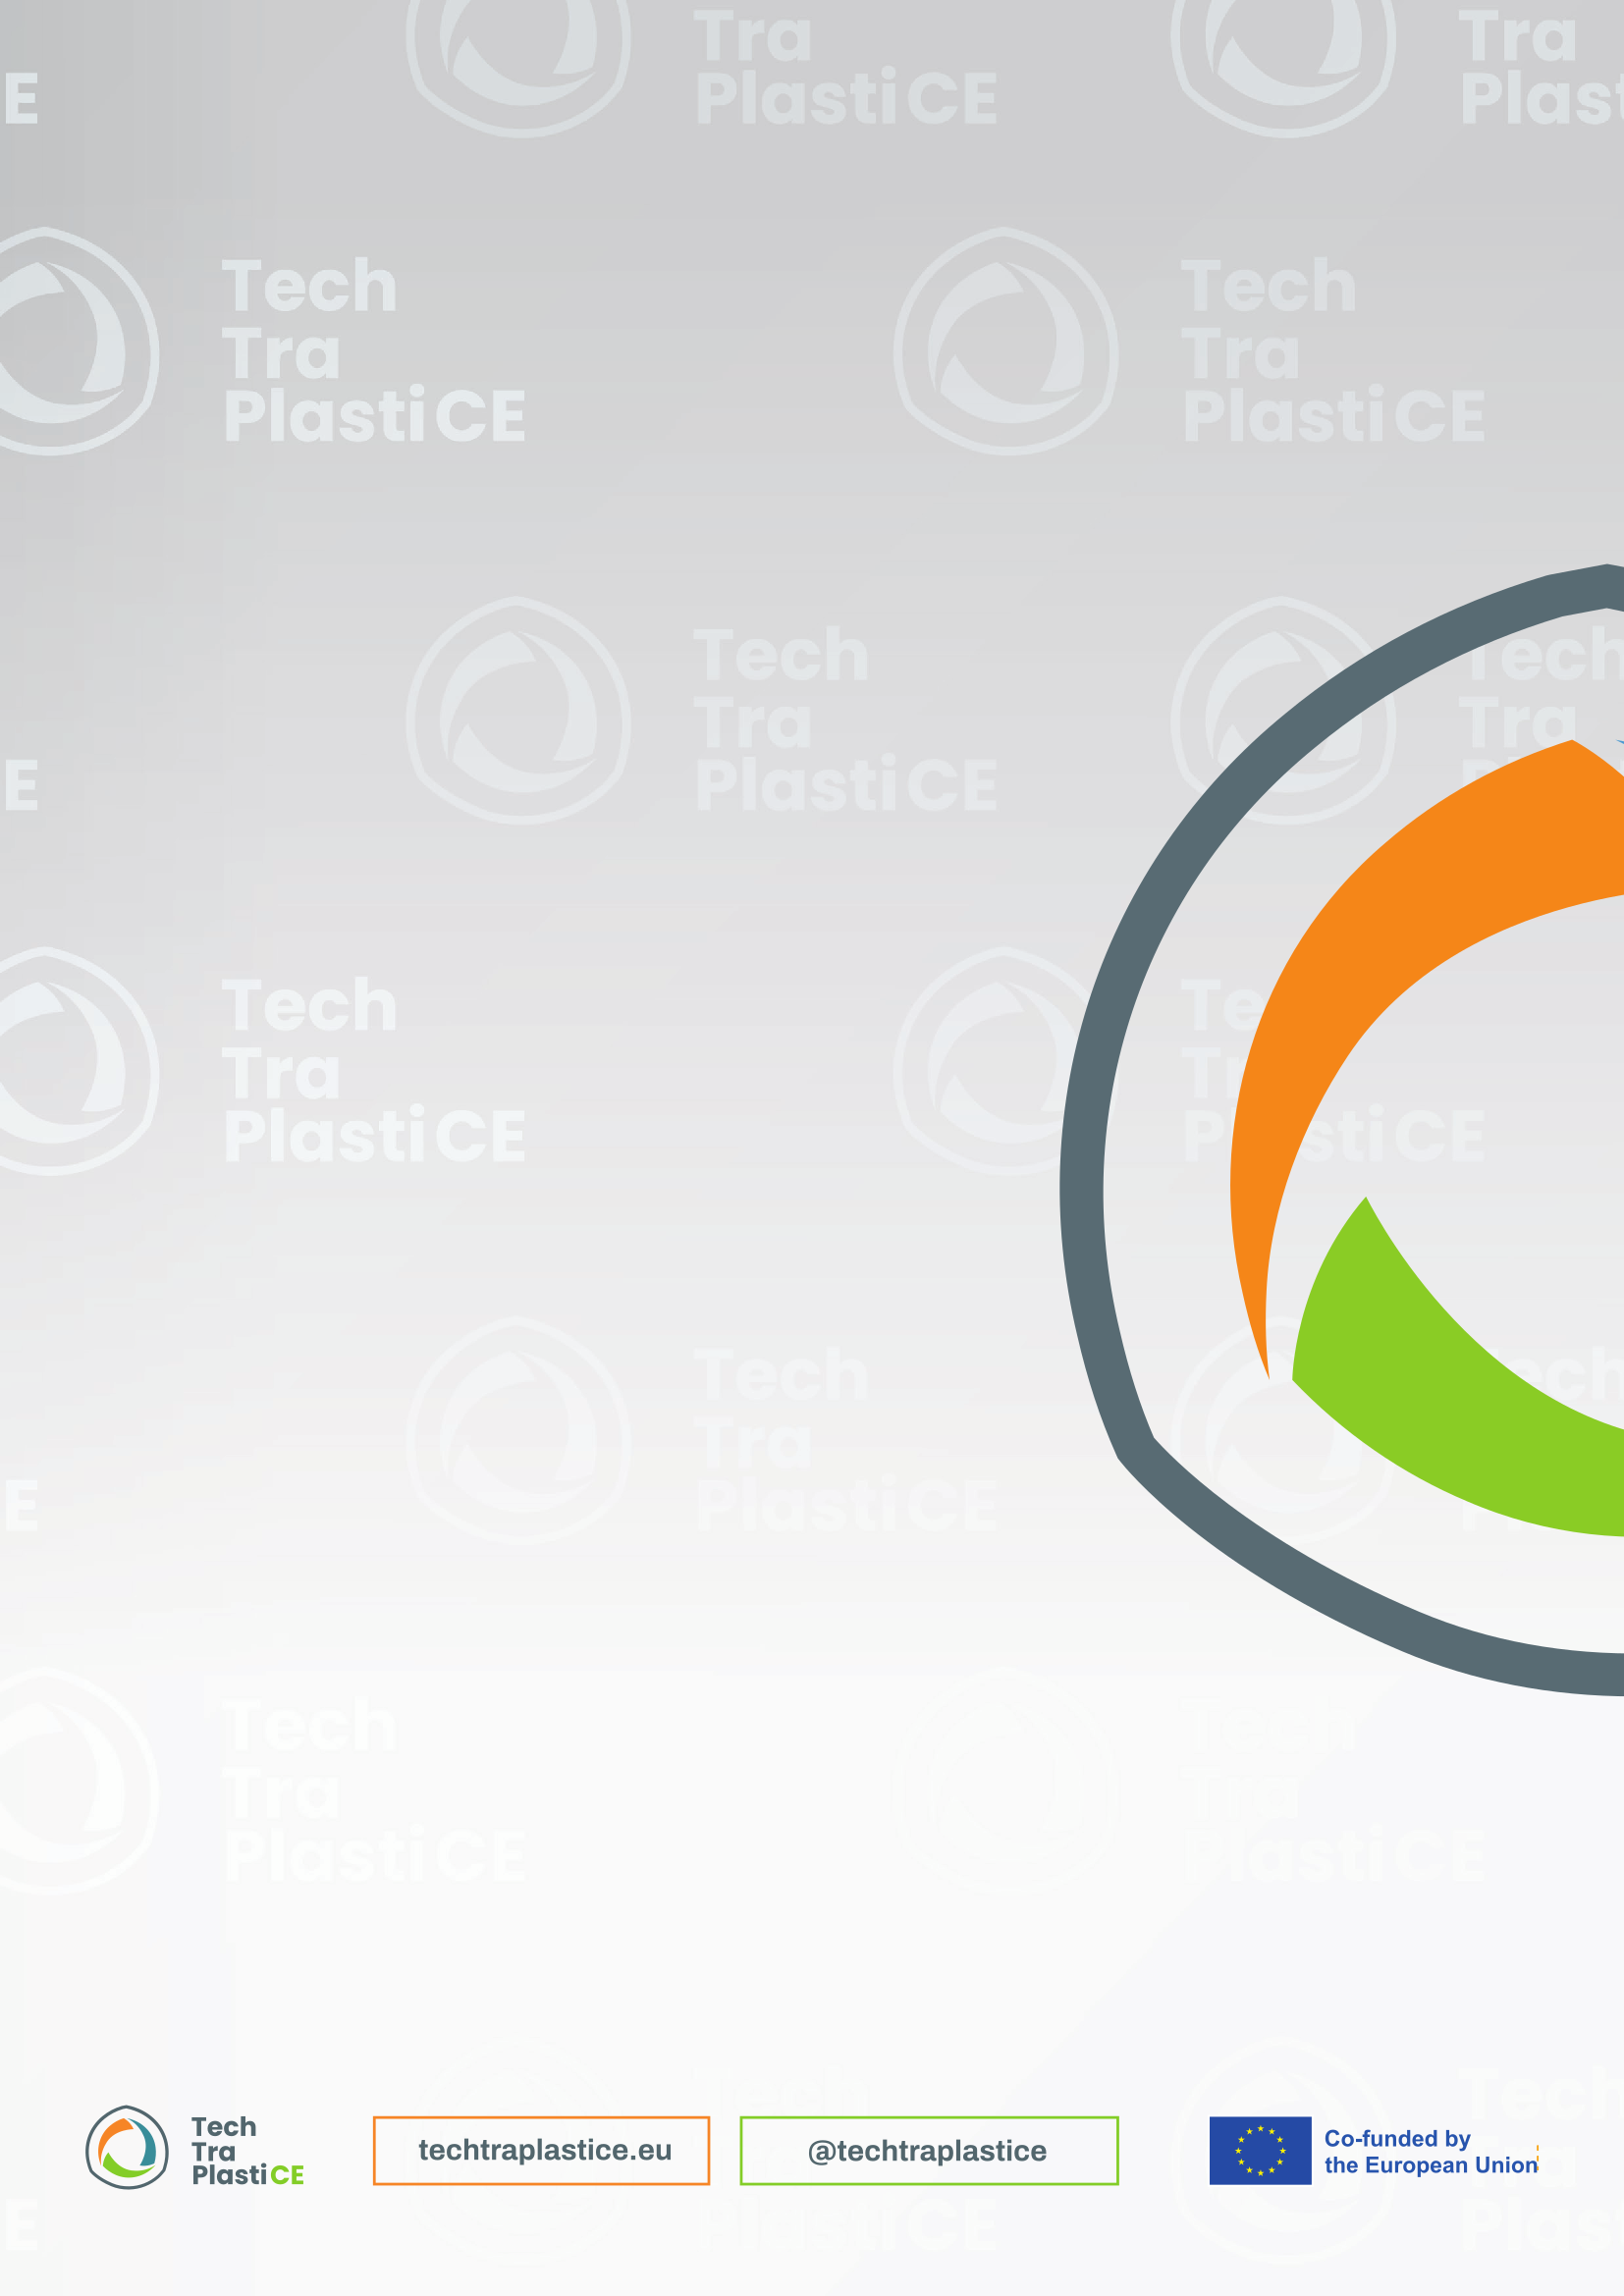
\includegraphics{assets/Portada.png}}
      }

  \BgThispage


  \begin{minipage}[b][0.78\textheight][s]{0.65\textwidth}

    \raggedright
    % Title and subtitle
    
    \vfill

    \begin{spacing}{2.2}
      {\color{Naranja}\Huge\bfseries{D2.3 Mentoring and
  peer-collaboration learning reports}} \\[1\baselineskip] 
    \end{spacing}
    
    \begin{spacing}{1.2}
    {\color{Neutro} \Large\textit{WP2: Development of a networked
  portfolio}}\\[1\baselineskip]
    
    {\Large \color{Neutro} 
    Strengthening University Tech Transfer Capabilities to Support Circular Economy 
    Value Chains for Plastics in Latin America -
    \textsc{\centering\bfseries TechTraPlastiCE} }\\[2\baselineskip]

    
    \end{spacing}

    {\color{Neutro} \Large\textit{November 25, 2026}}
    
    \vfill
  \end{minipage}		

  \vfill

  {\scriptsize
    \color{Neutro}
    This project has been funded with the support of Erasmus +.  
    The contents are the responsibility of the author(s). 
    The Commission cannot be held responsible for any use which may be made of the information contained therein. 
    Project No. 101179564 
    }


  \newpage



  \thispagestyle{plain}
  \begin{tabu} to \linewidth {X[1.3,l]  | X[1,l] X[1,l]}
    \toprule
    \multirow{5}{*}{ 
\includegraphics[height=20mm]{assets/images/logo-TTPCE.png}} &  \textbf{Work Package} : & WP2  \\ \cmidrule{2-3}
      & \textbf{Project Number} : & 101179564  \\ \cmidrule{2-3}
      &  \textbf{Type of document}:  & Deliverable   \\ \cmidrule{2-3}
      & \textbf{Due Delivery Date}:    & April
  30/2026     \\ \cmidrule{2-3}
      & \textbf{Actual Delivery Date}:    & November 25, 2026       \\ 
    \bottomrule
  \end{tabu}

  \vfill


  \begin{tabu} to \linewidth {X[1,l]  | X[3.5,l]}
    \toprule
    \textbf{Title} : & D2.3 Mentoring and peer-collaboration learning
  reports  \\ \cmidrule{2-2}
    \textbf{Work Package} : & WP2: Development of a networked
  portfolio  \\ \cmidrule{2-2}
    \textbf{Description} : & This repository will consist of digital
  memory on the cross-matching opportunities and
  initiatives.  \\ \cmidrule{2-2}
    \textbf{Responsible} : & Universidad Nacional del Sur \&
  Universidade de Aveiro  \\ \cmidrule{2-2}
    \textbf{Author(s)} : &  
     
          Prof.~Paula Ferreira (UA), Prof.~Idalina José Gonçalves (UA),
          Prof.~Cláudia Nunes (UA).
          
          Prof.~Yamila Victoria Vazquez (UNS), Prof.~Yanela N. Alonso
          (UNS), Prof.~Luciana A. Castillo, (UNS), Econ. Yesica Soledad
          Dilernia (UNS), ID. Teresa Dutari (UNS).
          
          PhD. Catalina Suescun (UL), Prof.~Fabio Cruz (UL).
           \\ \cmidrule{2-2}
    \textbf{Project Call} : & ERASMUS-EDU-2024-CBHE (Capacity building in the field of higher education)  \\ \cmidrule{2-2}
    \textbf{Dissemination Level} : & Confidential\\   
  \bottomrule
  \end{tabu}



  \vfill


  \begin{tabular}{ >{\raggedright\arraybackslash}p{3cm}| p{2cm} p{4cm} p{6cm} }
    \toprule
    \textbf{Version}: & \multicolumn{3}{l}{ 1.2} \\ \midrule
    \textbf{Contributors}  & Versions    & Dates       & Revision Description \\ \midrule
    UNS  & 1    & 23/04/2026  & Version 1 of the D.2.3 deliverable  \\ 
    UA  & 1.1    & 29/04/2026  & Consolidated document and feedback on the results.  \\ 
    UL  & 1.2   & 06/05/2026  & Final revision and integration of all feedback  \\ 
    \bottomrule
\end{tabular}  


    
    
    \vfill
    
    {\scriptsize\centering\color{lightgray} 
    
    Disclaimer
    
    This document is provided <<as is>> with no warranties whatsoever, 
    including any warranty or merchantability, non-infringement, fitness for any particular 
    purpose, or any warranty otherwise arising out of any proposal, specification or sample.  
    
    No license, express or implied, by estoppels or otherwise, to any intellectual 
    property rights are granted herein. 
    The members of the project TechTraPlastiCE do not accept any liability for actions or 
    omissions of TechTraPlastiCE members or third parties and disclaim any obligation 
    to enforce the use of this document. 
    
    This document reflects only the authors' view and the Commission is not responsible 
    for any use that may be made of the information it contains.  
    This document is subject to change without notice. 
    
    }
    \normalsize
    
    
    
      \end{titlepage}
  \end{frontmatter}

\renewcommand*\contentsname{Contents}
{
\setcounter{tocdepth}{2}
\tableofcontents
}
\listoffigures
\listoftables

\setstretch{1.2}
\mainmatter
\chapter*{Executive summary}\label{executive-summary}
\addcontentsline{toc}{chapter}{Executive summary}

This document contains the deliverable \textbf{D2.3 Mentoring and
peer-collaboration learning reports} of the \emph{Work Package 2 (WP2)
Development of a networked portfolio} of the TechTraPlastiCE project.
The scope of this deliverable is to present the mentoring and
peer-collaboration activities developed within the TechTraPlastiCE
project to strengthen technology transfer and circular economy
capacities among partner Higher Education Institutions (HEIs). Building
on the institutional portfolios created in Deliverables D2.1 and D2.2,
the report shifts the focus from mapping institutional capabilities to
activating them through collaborative learning, mentoring, and
inter-university exchange.

The methodology is based on a participatory, qualitative, and iterative
approach combining canvas-based institutional analysis, peer-learning
workshops, consortium meetings, and external expert validation.
Universities jointly identified strengths, needs, and opportunities for
cooperation across areas such as infrastructure, applied research,
innovation services, industry engagement, and training. This process
enabled the detection of complementary institutional profiles and the
creation of potential collaboration pathways within the consortium.

A central component of the deliverable is the contribution of the
External Advisory Board (EAB), composed of international experts in
innovation, entrepreneurship, sustainability, and technology transfer.
Their recommendations highlighted the importance of long-term strategic
coordination, institutional flexibility, and stronger links between
academia, industry, and society. Overall, D2.3 demonstrates how
network-based collaboration and mentoring can enhance institutional
learning, improve technology transfer practices, and support the
development of sustainable innovation ecosystems in the plastics
circular economy sector.

\chapter{Introduction}\label{introduction}

Building on the results of D2.1 and D2.2, which enabled the structuring
of institutional portfolios and the characterization of technology
transfer capacities across the consortium universities, this deliverable
focuses on activating these capacities through \emph{cross-peer
collaboration and mentoring processes among partner institutions}. While
D2.2 provided a structured and comparable understanding of institutional
strengths, profiles, and transfer orientations, the effective
implementation of these portfolios requires moving beyond individual
institutional analysis towards joint and collaborative dynamics. In this
context, HEI are not only knowledge providers but also active
participants in shared learning processes, where experiences,
methodologies, and practices can be transferred and adapted across
different institutional and regional contexts.

Within this framework, D2.3 aims to foster cross-peer collaboration and
mentoring activities that enable more experienced partners to share
practices related to the delivery of solutions, services, and
methodologies for portfolio implementation. This process seeks to create
matching opportunities among institutions, allowing them to advance
according to their specific needs, capacities, and strategic priorities.
To support this process, an External Advisory Board (EAB) was
established, composed of experts selected through a collaborative
process among partner institutions. Each university proposed
professionals with relevant experience aligned with the focus of the
project, ensuring a diverse and complementary set of perspectives in
areas such as technology transfer, innovation, sustainability, and
industry engagement.

The present deliverable presents an integral analysis of the portfolios,
member profiles, and EAB perspectives, in order to combine internal
reflection, collective analysis, and external feedback. This analysis
allowed to identify complementarities, shared challenges, and
opportunities for collaboration. In this sense, D2.3 contributes to
bridging the gap between structured knowledge (institutional portfolios)
and actionable collaboration, reinforcing the role of the consortium as
a dynamic network capable of co-developing solutions and scaling impact
in the field of plastic circular economy.

\begin{figure}[H]

\centering{

\pandocbounded{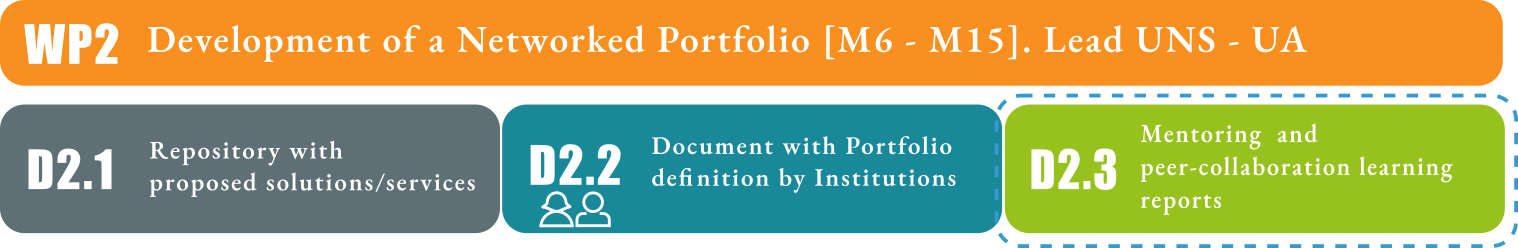
\includegraphics[keepaspectratio,alt={alt}]{figures/2.3/D2.3.png}}

}

\caption{\label{fig-baseline}Mentoring and peer-collaboration for
TechTraplastiCE Project}

\end{figure}%

\chapter{Methodological Approach}\label{methodological-approach}

The methodological approach adopted in this deliverable is based on a
participatory, qualitative, and iterative process aimed at fostering
peer-learning, mentoring, and collaboration among partner institutions.
It integrates internal analysis, collective reflection, and external
validation to support the transition from institutional portfolios to
collaborative implementation strategies.

\section{Canvas-based institutional
analysis}\label{canvas-based-institutional-analysis}

As it was presented in D2.1, a key activity was conducted during the
consortium meeting held in Chile during November 2025, where the nine
partner universities participated in a structured exercise based on the
canvas methodology. his activity aimed to map institutional capacities
related to knowledge and technology transfer and to identify
opportunities for inter-university collaboration.

The exercise was structured around eight analytical blocks:

\begin{enumerate}
\def\labelenumi{\arabic{enumi}.}
\tightlist
\item
  Human and organizational capacities,
\item
  Infrastructure and equipment,
\item
  Applied R\&D results,
\item
  Technological services and developments,
\item
  Training and education,
\item
  Institutional engagement strategies,
\item
  Barriers and opportunities, and
\item
  Inter-university collaboration opportunities
\end{enumerate}

Guiding questions (Figure~\ref{fig-canva}) were used to stimulate
reflection on institutional strengths, available resources, transfer
potential, interaction mechanisms with external stakeholders, and key
challenges. While blocks 1 to 7 informed the characterization of
institutional profiles (submitted via the Google Forms described in D2.1
and analyzed in D2.2), \textbf{block 8 focused specifically on
identifying complementarities and opportunities for collaboration. This
component was further developed through a dedicated follow-up form
completed by each institution.}

\begin{figure}[H]

\centering{

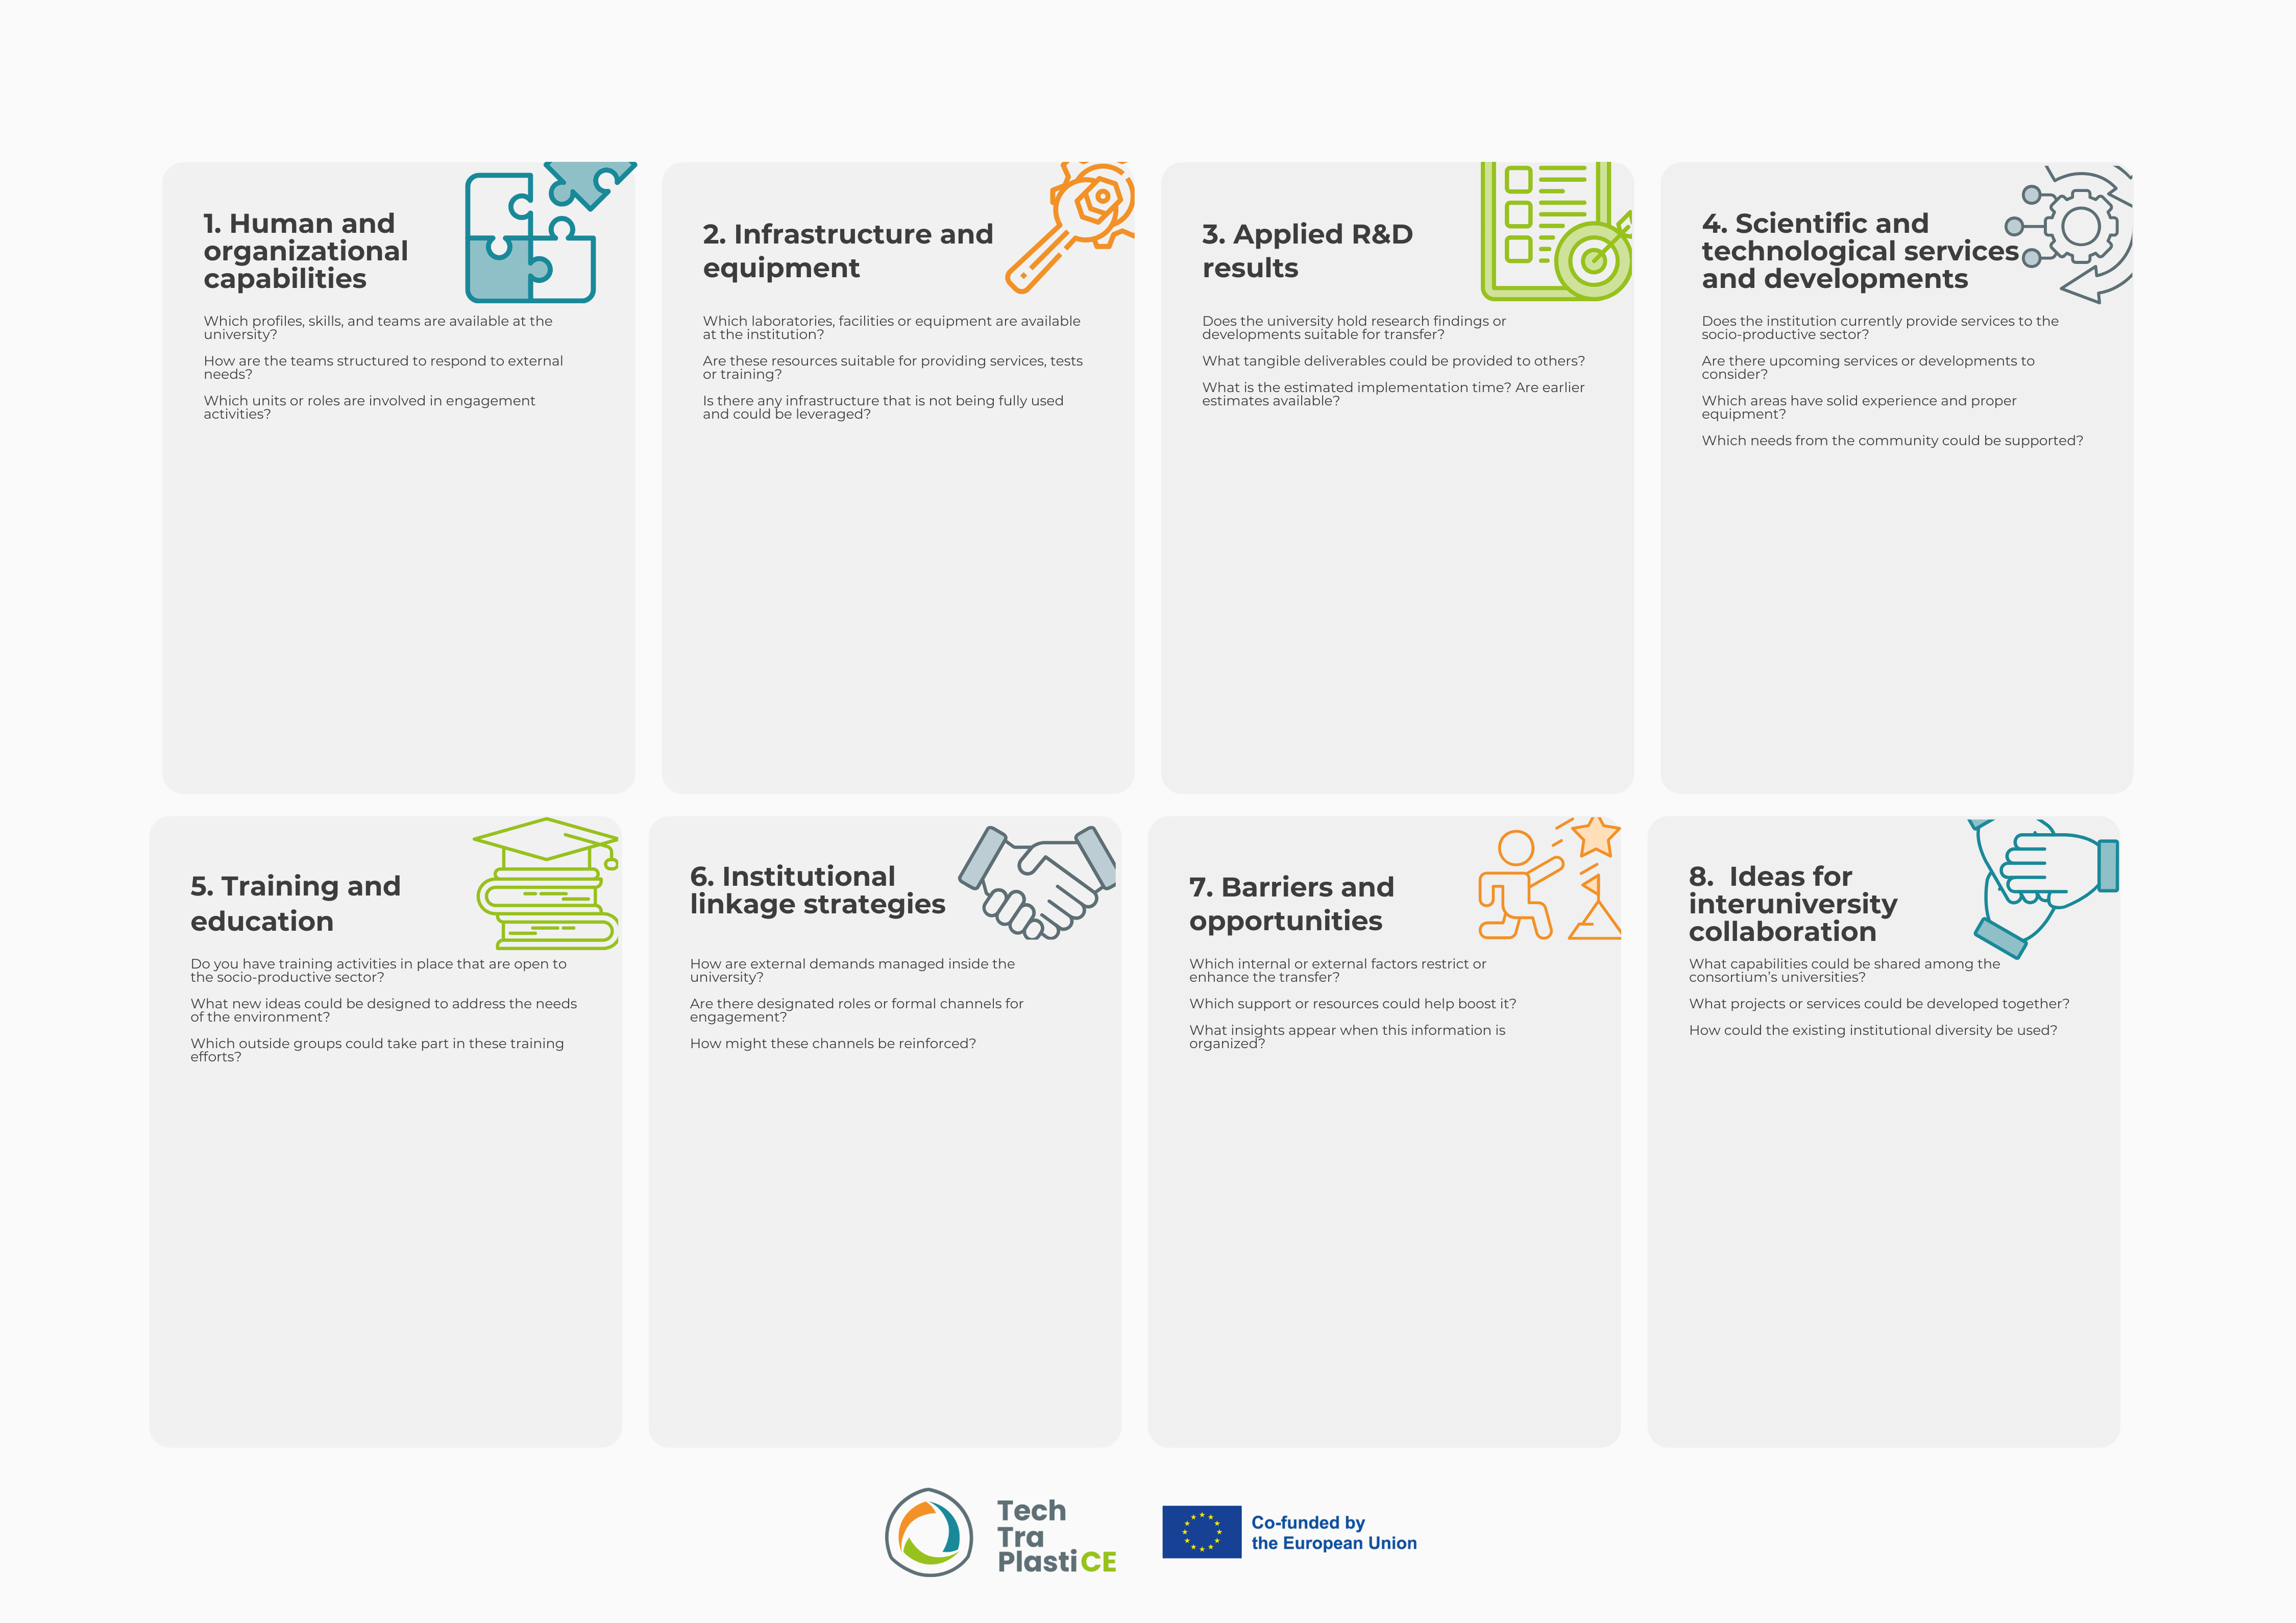
\includegraphics[width=1\linewidth,height=\textheight,keepaspectratio]{figures/2.1/Canva.png}

}

\caption{\label{fig-canva}Canva used at the workshop at the meeting
consortium in Chile Nov 2025}

\end{figure}%

In addition to the canvas-based mapping exercise, a complementary
perspective mentoring based on \emph{open innovation} was incorporated
through a subsequent virtual session at the general meeting of the
consortium in December 2066. This approach aimed to enrich the
analytical framework by introducing collaborative and co-creation
dynamics as a key dimension of technology transfer processes from the
presential meeting made at Chile in Nov.~2025 (See the presentation in
the Annex).

\begin{figure}[H]

\centering{

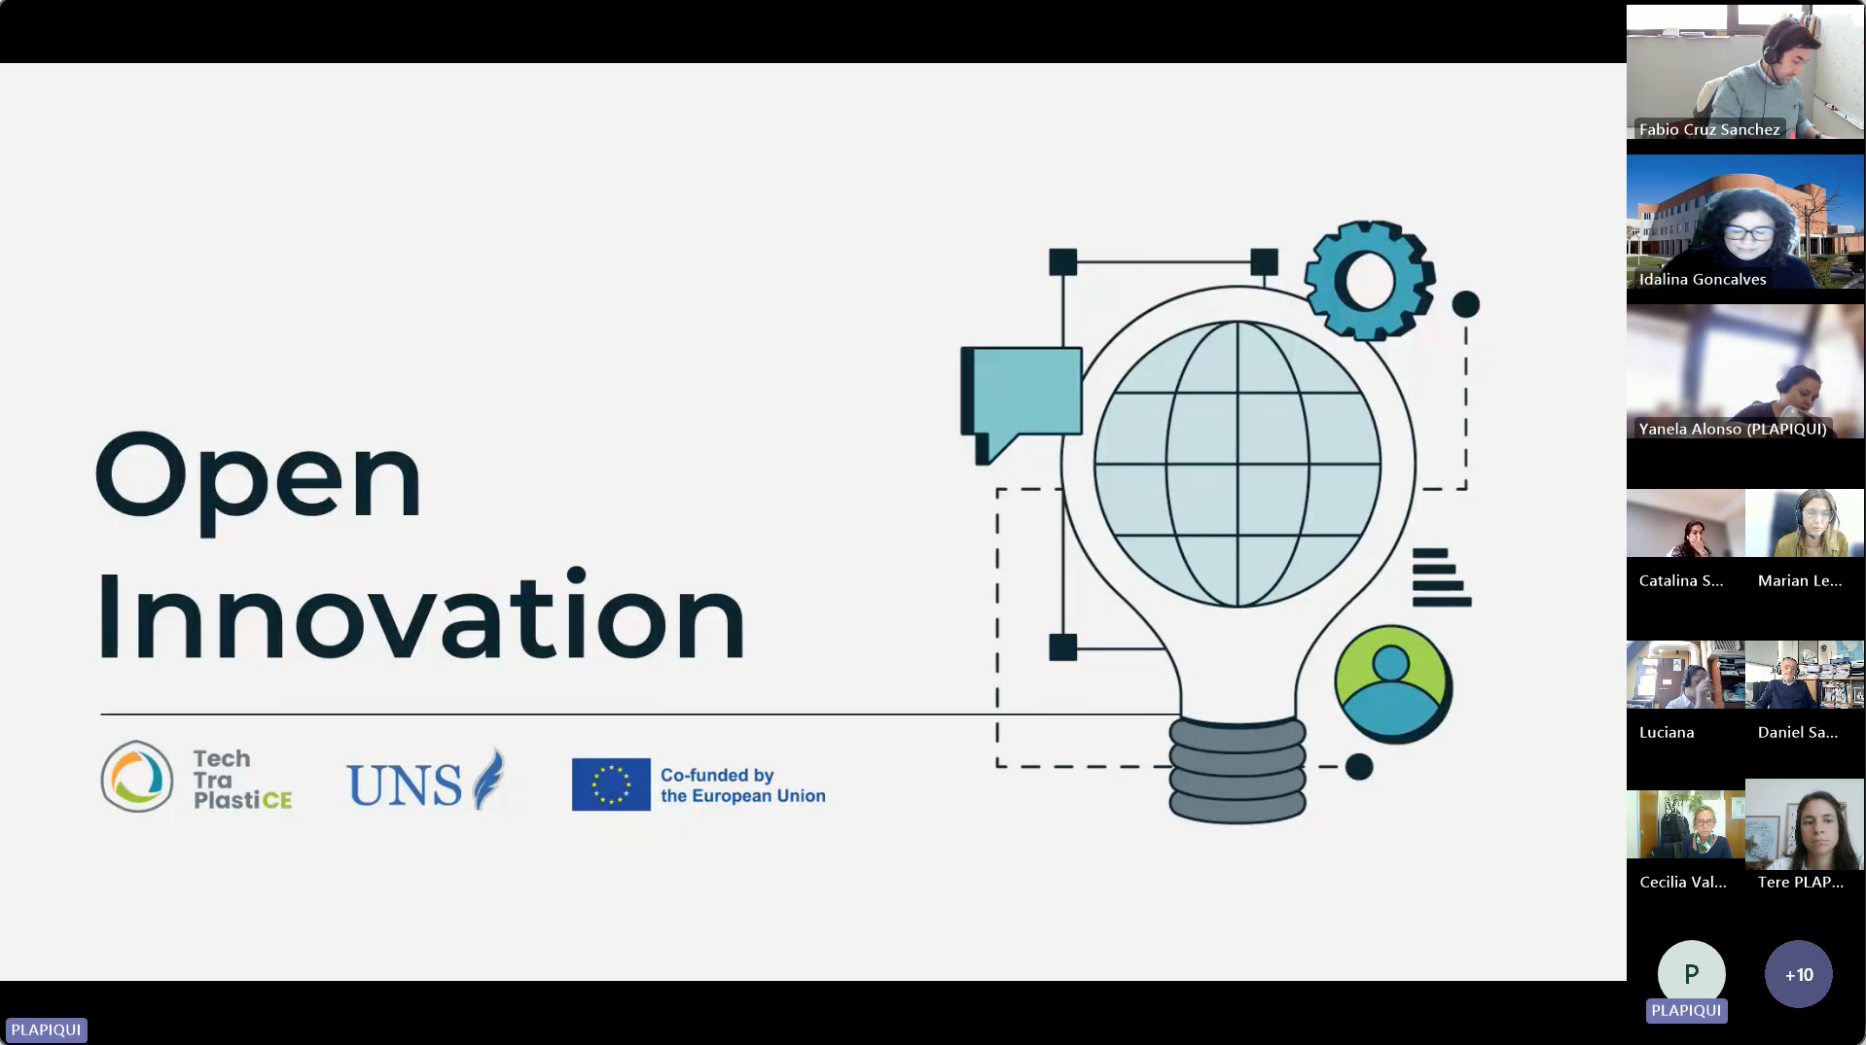
\includegraphics[width=0.95\linewidth,height=\textheight,keepaspectratio]{figures/2.3/Open-inno.png}

}

\caption{\label{fig-open}Presentation on Open Innovation made by the UNS
at the General meeting of December 2025}

\end{figure}%

From a methodological standpoint, the integration of open innovation
allowed to move beyond a static identification of institutional
capacities towards a more dynamic understanding of how these capacities
can be mobilized, in interaction with external stakeholders. In
particular, it introduced a shift from linear models of technology
transfer (based on predefined demands) towards iterative and
collaborative processes, where problems and solutions are jointly
defined and developed. As a result, the combined use of the canvas
methodology and the open innovation perspective provided a more
comprehensive framework to analyze not only what institutions can offer,
but also how these capacities can be articulated within collaborative
ecosystems, both within the consortium and in relation to external
actors.

\section{External Advisory Board workshop and structured
exchange}\label{external-advisory-board-workshop-and-structured-exchange}

A second core component of the methodology was the interaction with the
EAB. During the second semester of 2025, the members of the EAB made a
official presentation to the TechTraPlastiCE consortium on topic related
to the technology transfer and Circular Economy. Then, a virtual
workshop with most of the EAB was carried out through on March 26th,
2026. The composition of the EAB reflects the diversity of expertise
required to address technology transfer challenges within the circular
economy of plastics, combining academic, industrial, and strategic
perspectives. The workshop aimed to deepen the understanding of
institutional barriers and opportunities, and to obtain strategic
recommendations for strengthening technology transfer practices.

The session was structured into four blocks:

\begin{itemize}
\tightlist
\item
  Contextualization of the project and institutional environments,
\item
  Short presentations by each university based on a structured pitch
  format,
\item
  Guided discussion with EAB members to identify patterns, differences,
  and opportunities and,
\item
  Final synthesis with strategic recommendations.
\end{itemize}

Each institution presented its context, key challenges, and planned
actions for the following 12 months, focusing on implementation
strategies rather than descriptive reporting.

\section{Identification of complementarities and matching
opportunities}\label{identification-of-complementarities-and-matching-opportunities}

The combination of the canvas analysis and the EAB workshop enabled the
identification of complementarities across institutions, forming the
basis for cross-peer collaboration and mentoring.

The analysis focused on:

\begin{itemize}
\tightlist
\item
  Identifying areas of affinity (shared thematic interests),
\item
  Detecting complementarities (where capacities can be combined) and,
\item
  Recognizing potential mentoring dynamics based on different levels of
  experience and maturity.
\end{itemize}

This approach allowed the transition from individual institutional
portfolios to a network-based perspective, where collaboration is
understood as a key mechanism for enhancing the effectiveness and
scalability of technology transfer activities.

\chapter{Results and Discussion}\label{results-and-discussion}

\section{External Advisory Board
participation}\label{external-advisory-board-participation}

As part of the cross-peer learning and validation process, an EAB was
established during 2025 (\emph{c.f. D6.1. Quality assurance plan}),
composed of experts with relevant experience in technology transfer,
innovation, sustainability, and industry engagement. The members of the
EAB were proposed by the partner institutions, ensuring a diverse and
complementary representation aligned with the focus of the project. The
EAB played a key role in providing external insights, identifying common
challenges across institutions, and contributing strategic
recommendations to strengthen the implementation of institutional
portfolios.

\subsection{Ferran Giones}\label{ferran-giones}

Deputy Director of the Institute for Entrepreneurship and Innovation
Science (ENI) at the University of Stuttgart (Germany), and has
previously served as Adjunct Professor of Technological Entrepreneurship
at the University of Southern Denmark (SDU). His expertise centers on
technological entrepreneurship and the processes underlying industrial
emergence, with a particular focus on the interplay between startups,
established firms, and emerging technologies. His work also addresses
the commercialization of scientific knowledge, examining how new
technologies are translated into viable applications. In addition, he
has developed contributions in the field of technological exaptation,
analyzing how existing technologies are repurposed within innovation
strategies across both entrepreneurial ventures and established
organizations.

\subsection{María José Zapata}\label{maruxeda-josuxe9-zapata}

Associate Professor at the Faculty of Economics, Law and Business at the
University of Gothenburg since 2017. Her expertise lies in the
foundations of sustainability, with a particular focus on the design and
governance of public--private partnerships, the organizational
dimensions of sustainability, and the structuring of environmental
sustainability initiatives in urban contexts. Her work addresses how
institutions coordinate, manage, and implement sustainability
strategies, contributing to a deeper understanding of governance models
and collaborative mechanisms for sustainable urban development.

\subsection{Astrid Jaime - Associate Researcher at the Universidad
Minuto de Dios in
Colombia}\label{astrid-jaime---associate-researcher-at-the-universidad-minuto-de-dios-in-colombia}

At the monthly general consortium of TechTraPlastiCE of Oct.~2025,
Prof.~Jaime presented her expertise research on innovation project
management, knowledge transfer processes, entrepreneurship, and
intellectual property as illustrated Figure~\ref{fig-UIS}. She has
extensive experience in teaching and outreach activities related to
these fields, contributing to the dissemination and application of
knowledge. THe TechTraPlastiCE consortium could have on overview of her
work which is centered on the articulation of science, technology, and
innovation systems, with a particular focus on knowledge management and
its role in strengthening institutional and socio-productive linkages.

\begin{figure}

\begin{minipage}[t]{0.47\linewidth}

\begin{figure}[H]

\centering{

\pandocbounded{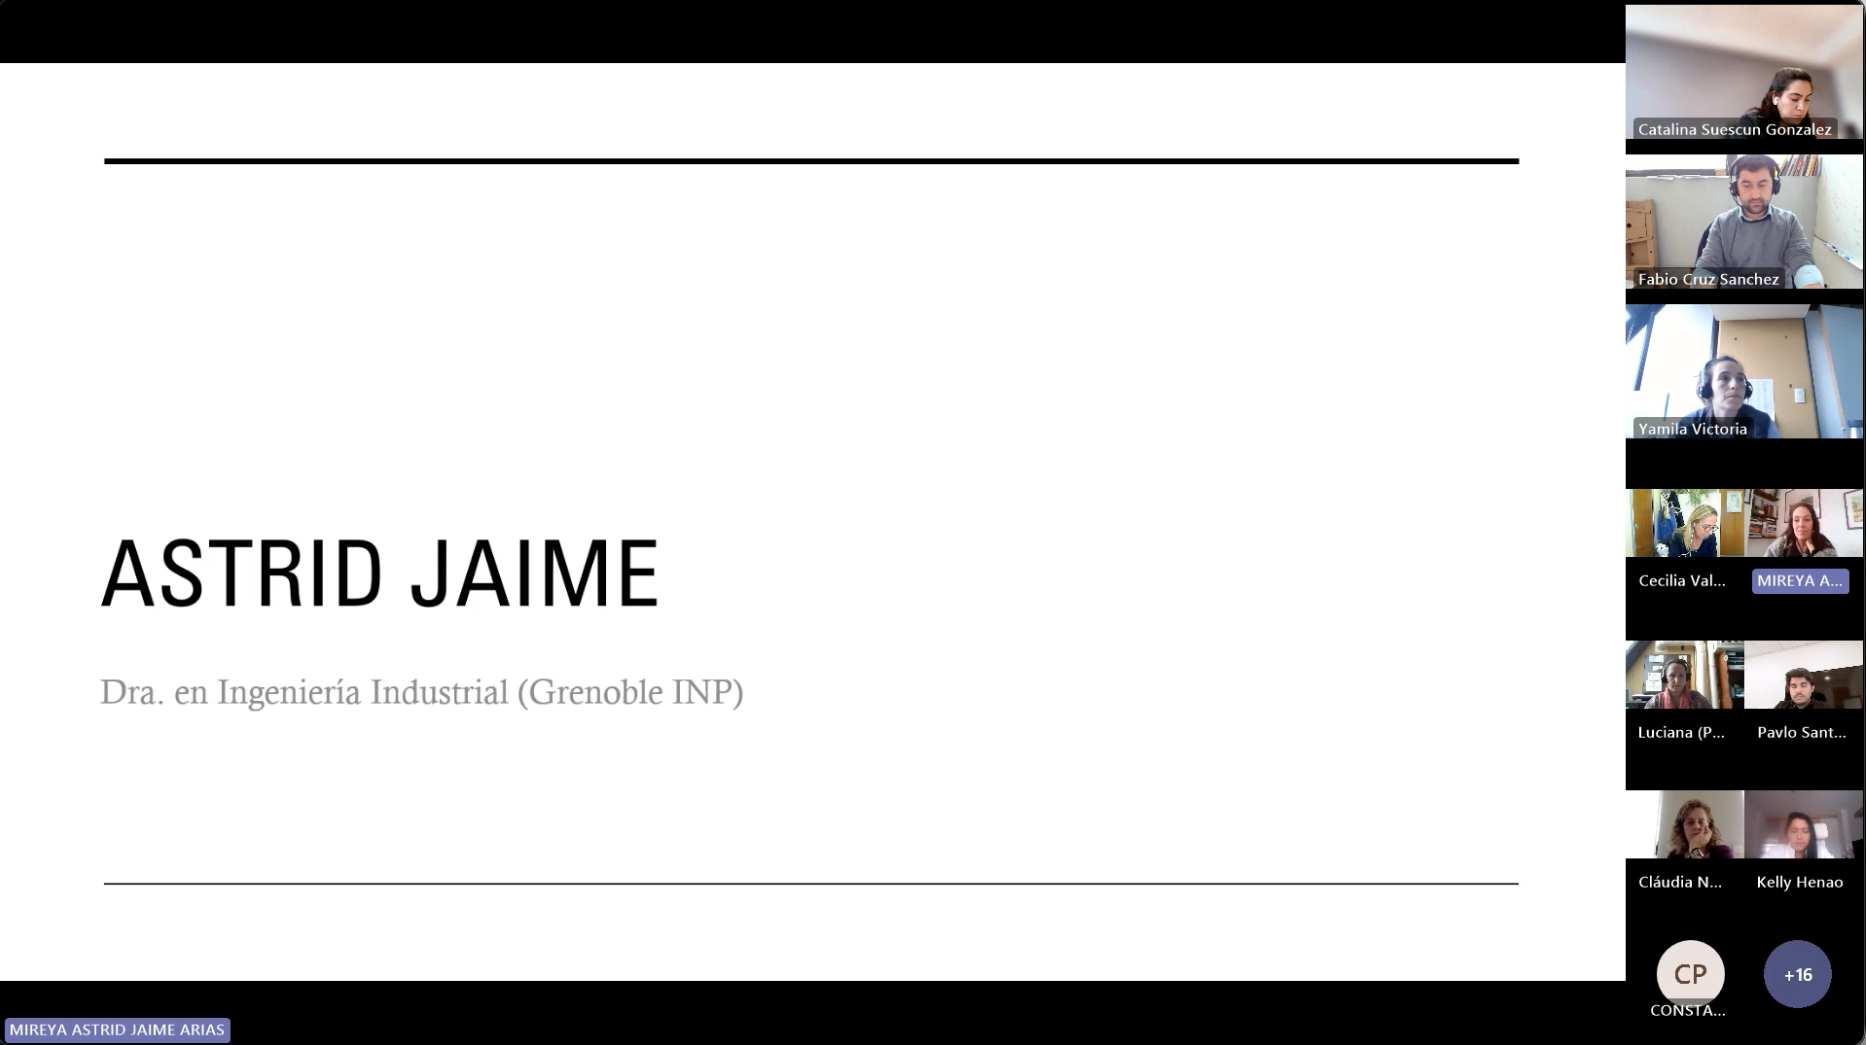
\includegraphics[keepaspectratio,alt={alt}]{figures/2.3/Astrid-00.png}}

}

\caption{\label{fig-id}Presentation of Prof.~Astrid Jaime to the
TechTraPlastiCE Consortium on general meeting of Oct.~2025}

\end{figure}%

\end{minipage}%
%
\begin{minipage}[t]{0.05\linewidth}
~\end{minipage}%
%
\begin{minipage}[t]{0.47\linewidth}

\begin{figure}[H]

\centering{

\pandocbounded{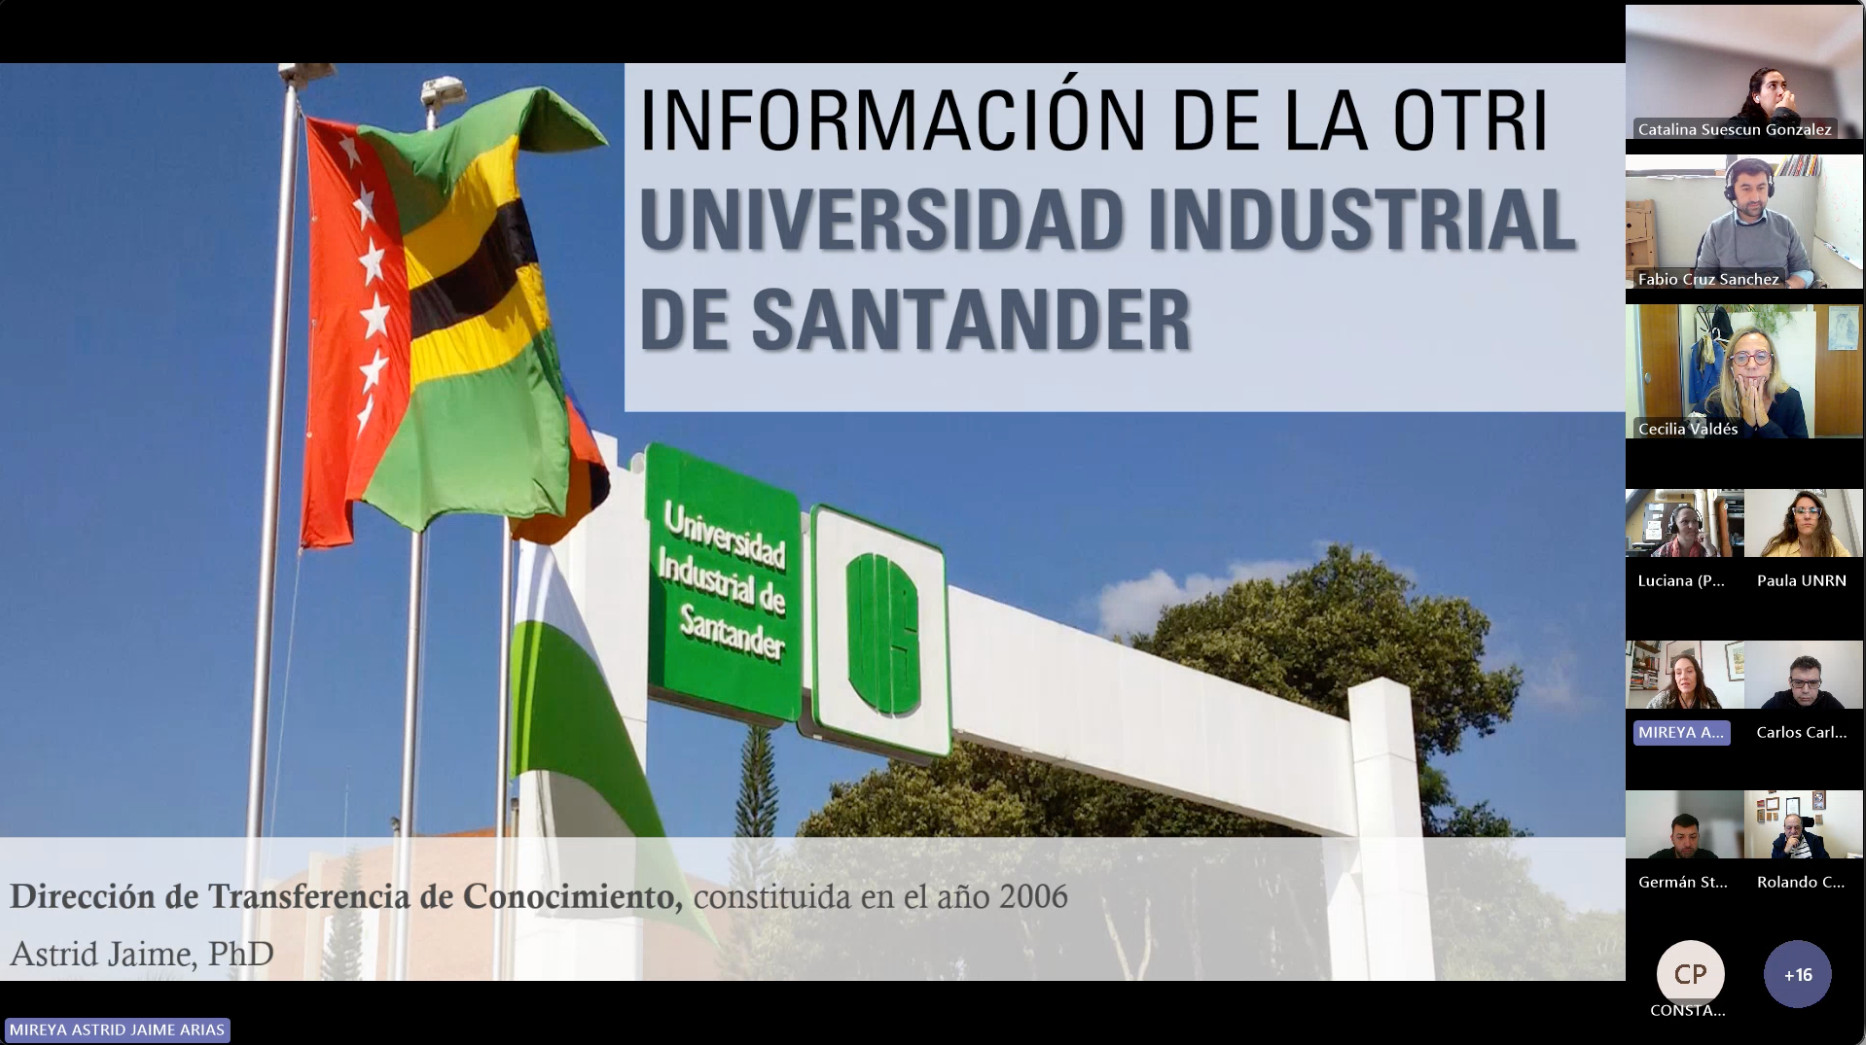
\includegraphics[keepaspectratio,alt={alt}]{figures/2.3/Astrid-01.jpg}}

}

\caption{\label{fig-UIS}Prof.~Astrid Jaime presented to the consortium
her experience on the Tech Transfer Office of the Universidad Industrial
de Santander}

\end{figure}%

\end{minipage}%

\end{figure}%

The major concrete shared experience of Prof.~Astrid Jaime was focalised
on all major problems and issues on the case of implementation the
Tech-Transfer office of Universidad Industrial of Santander in Colombia
in 2015. She gave a landscape from reglamentation issues to the
professor engagement in the activities related to the tech transfer in
the case of Colombia. These aspects elucidated the Colombian context and
the strategies that she and her team had to implement.

\subsection{Verónica Bucalá -- Co-founder of SophIA-X and Ex-Research
Director of PlaPiui - CONICET -
Argentina}\label{veruxf3nica-bucaluxe1-co-founder-of-sophia-x-and-ex-research-director-of-plapiui---conicet---argentina}

Véronica leads innovation initiatives and corporate training programs in
artificial intelligence, with a focus on the implementation of
responsible and applied solutions. She holds a PhD in Chemical
Engineering and has developed a distinguished career as a Principal
Investigator at CONICET, combining research, teaching, and scientific
leadership. She served as Director of PLAPIQUI (UNS--CONICET) and as
Dean of the Department of Chemical Engineering at the Universidad
Nacional del Sur.

\begin{figure}

\begin{minipage}[t]{0.47\linewidth}

\begin{figure}[H]

\centering{

\pandocbounded{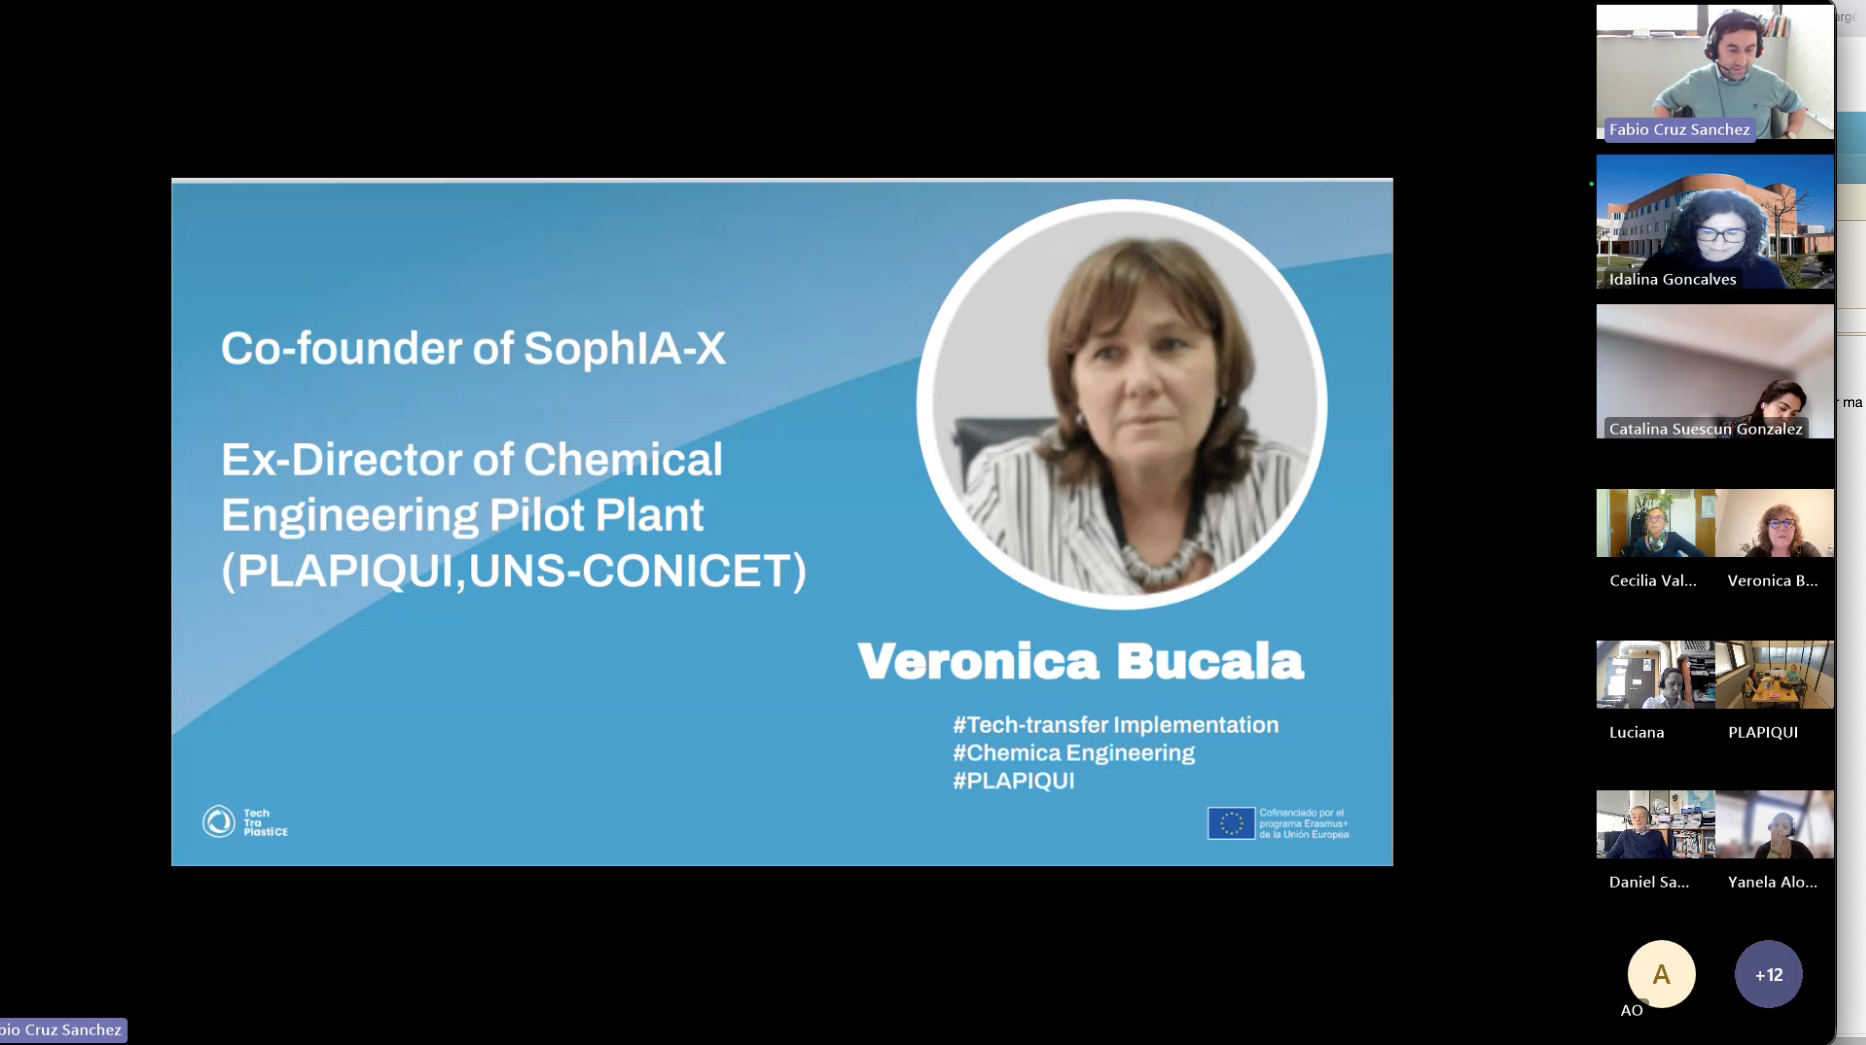
\includegraphics[keepaspectratio,alt={alt}]{figures/2.3/Veronica-00.png}}

}

\caption{\label{fig-id}Presentation of Ex-Prof.~Veronical Bucala to the
TechTraPlastiCE Consortium on general meeting of Dec.~2025}

\end{figure}%

\end{minipage}%
%
\begin{minipage}[t]{0.05\linewidth}
~\end{minipage}%
%
\begin{minipage}[t]{0.47\linewidth}

\begin{figure}[H]

\centering{

\pandocbounded{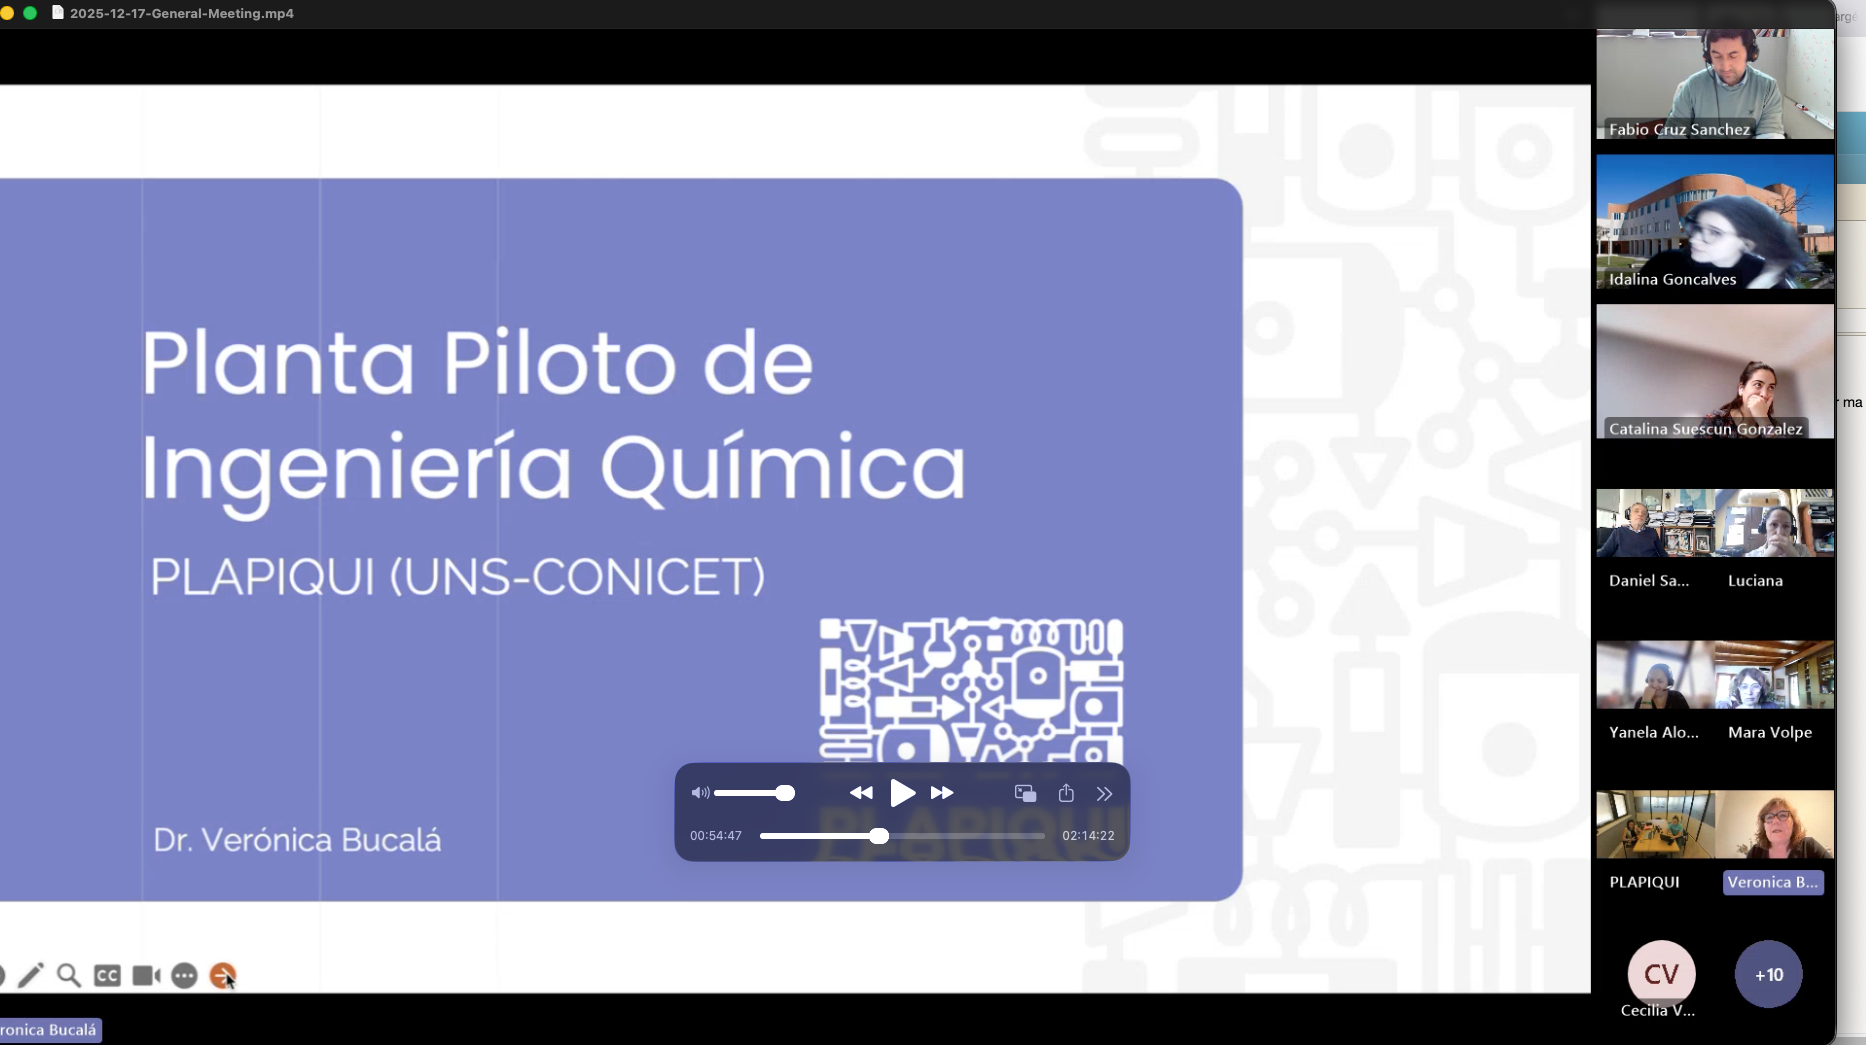
\includegraphics[keepaspectratio,alt={alt}]{figures/2.3/Veronica-01.png}}

}

\caption{\label{fig-UIS}Ex-Prof.~Véronica Bucala presented her
experience on the implementation of Tech Transfer Office at the ``Planta
Piloto de Ingenieria Quimica'' (Universidad Nacional del Sur)}

\end{figure}%

\end{minipage}%

\end{figure}%

On the monthly general meeting of TechTraPlastiCE in Dec.~2025, she
shared to the consortium her experience on the key role in strengthening
the link between science and industry and promoting technology transfer
processes. The major output of this session was to better understand the
value of her expertise on process engineering, innovation management,
for the articulation between academic knowledge and industrial
application. She gives insigths on the structuration of the portfolio of
chemical

This is important for the role that TechTraPlastiCE aims to look for
fostering Circular Economy in the plastic value chain. The engineering
domain plays in oustanding role in this transition.

\subsection{Mara Volpe -- Technical Director at Cyclus in
Argentina}\label{mara-volpe-technical-director-at-cyclus-in-argentina}

PhD. Mara Volpe leads the development of technology and consulting
services grounded in the principles of circular economy and
decarbonization.

She has over 30 years of experience as a scientific researcher, with
expertise in heterogeneous catalysis, biomass pyrolysis, biochar
production for steel and agricultural industries, and advanced chemical
recycling of mixed plastics and end-of-life tires.

Likewise ex-Prof.~Veronica Bucala, on the general meeeting of Dec.~2025,
TechTraPlastiCE consortium had the opportunity to understand the work of
Mara at the circular Economy start-up CYCLUS to understand the
decarbonization challenges including the extensive interdisciplinary
work across biology, agronomy, and electronic and mechanical
engineering, alongside strong collaboration with the private sector.

\begin{figure}

\begin{minipage}[t]{0.47\linewidth}

\begin{figure}[H]

\centering{

\pandocbounded{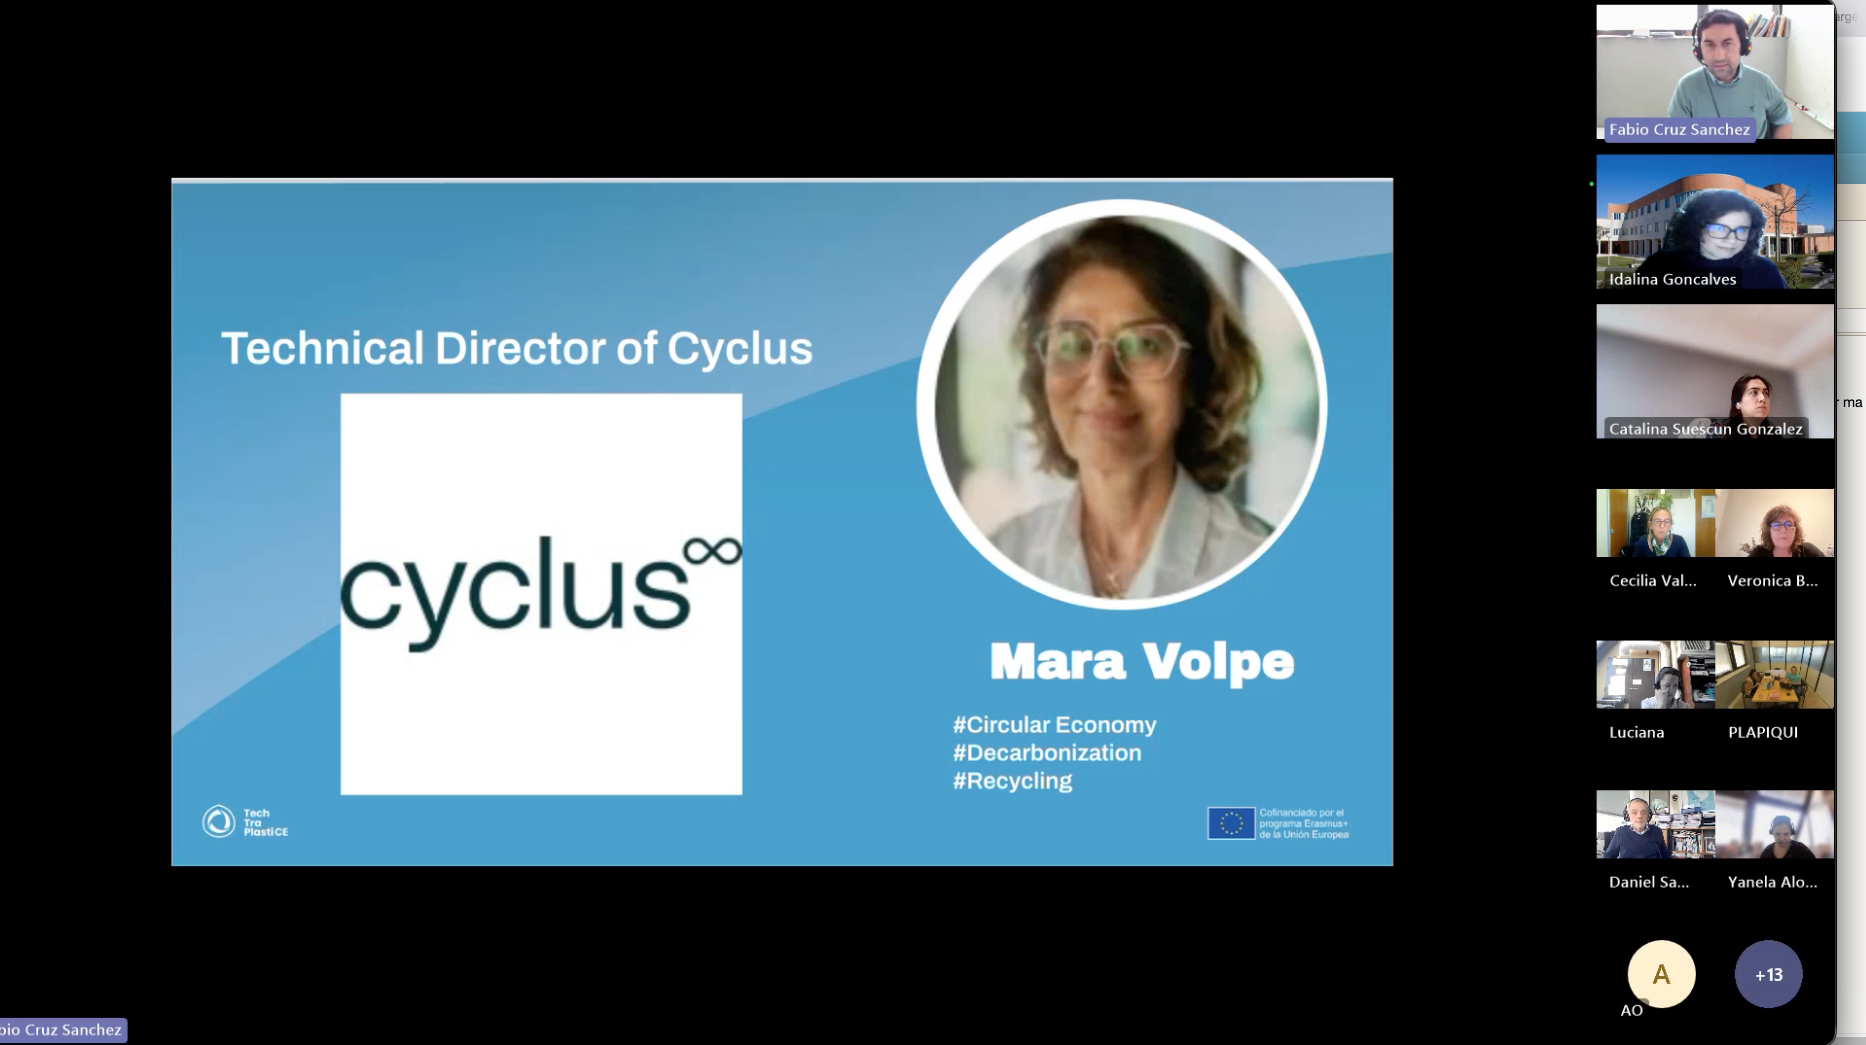
\includegraphics[keepaspectratio,alt={alt}]{figures/2.3/Mara-00.png}}

}

\caption{\label{fig-id}Presentation of PhD. Mara Volpe to the
TechTraPlastiCE Consortium on general meeting of Dec.~2025}

\end{figure}%

\end{minipage}%
%
\begin{minipage}[t]{0.05\linewidth}
~\end{minipage}%
%
\begin{minipage}[t]{0.47\linewidth}

\begin{figure}[H]

\centering{

\pandocbounded{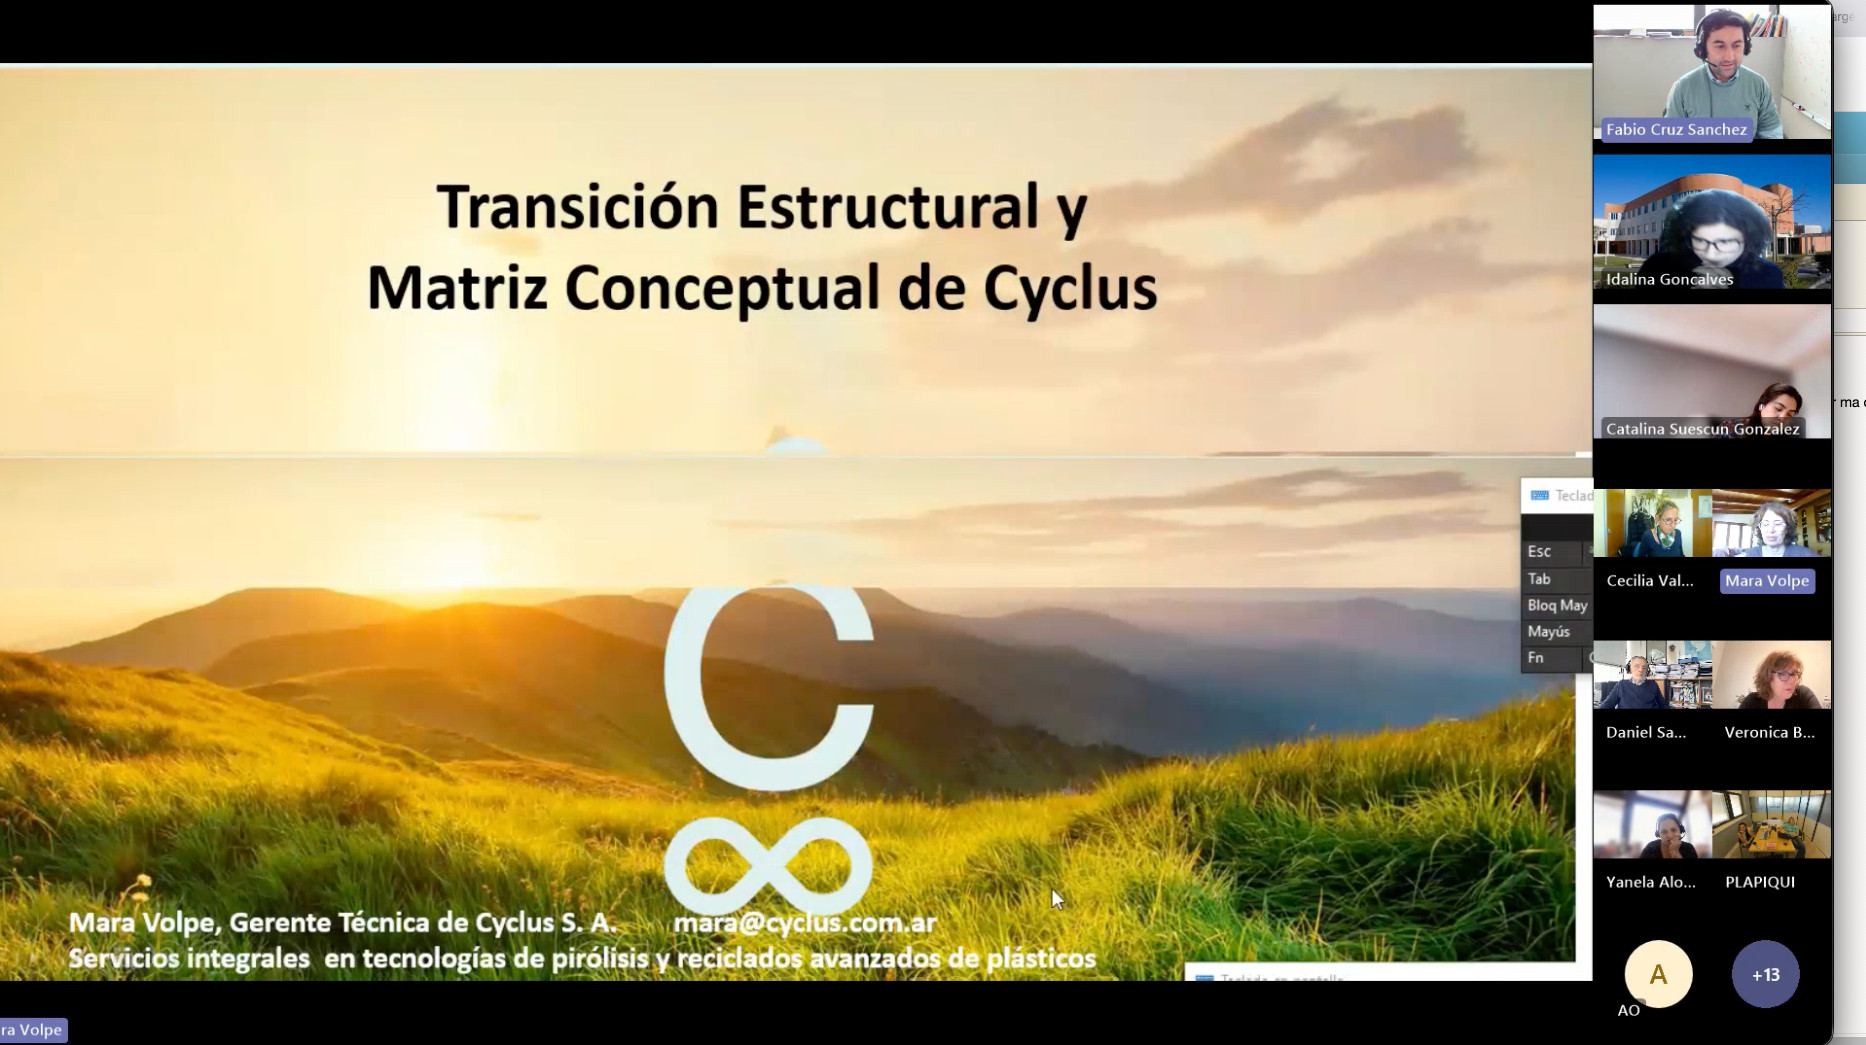
\includegraphics[keepaspectratio,alt={alt}]{figures/2.3/Mara-01.jpg}}

}

\caption{\label{fig-UIS}PhD. Mara Volpe presented her experience on the
start-up \href{https://cyclus.com.ar/}{CYCLUS - https://cyclus.com.ar/}
on circular economy issues}

\end{figure}%

\end{minipage}%

\end{figure}%

She presented her work focusing on the design and implementation of
projects based on a triple bottom line approach, integrating social,
environmental, and economic dimensions to promote sustainable practices
and innovative solutions.

\subsection{Flavio Soldera -- General Manager of the European School of
Materials (EUSMAT) at the University of Saarland in
Germany}\label{flavio-soldera-general-manager-of-the-european-school-of-materials-eusmat-at-the-university-of-saarland-in-germany}

Flavio holds a PhD in Materials Science and Engineering and has over 25
years of experience in scientific research focused on advanced materials
for electrical applications, 3D analysis of micro- and nanostructures,
and the use of electron microscopy and focused ion beam techniques. He
also brings more than 20 years of experience in the coordination and
management of international research and education projects.

On the general meeting of April 2026, the TechTraplastiCE consortium had
the view of his work as part of Material Engineering Center Saarland
\url{https://www.mec-s.de/en/welcome-2/}, an institute dedicated to
technology transfer between academia and industry. We had the
opportunity to he has extensive expertise in collaborating with the
industrial sector, particularly in areas related to materials
characterization and applied research. More precisely, He presented the
\href{https://www.uni-gr.eu/fr/CIRKLA}{The European Interreg
UniGR-CIRKLA project -- https://www.uni-gr.eu/fr/CIRKLA} that brings
together science, industry, and society to accelerate the transition to
a circular economy for metals and materials in the Greater Region
(Lorraine - Wallonia - Saarland - Luxembourg - Rhineland-Palatinate).

\begin{figure}

\begin{minipage}[t]{0.47\linewidth}

\begin{figure}[H]

\centering{

\pandocbounded{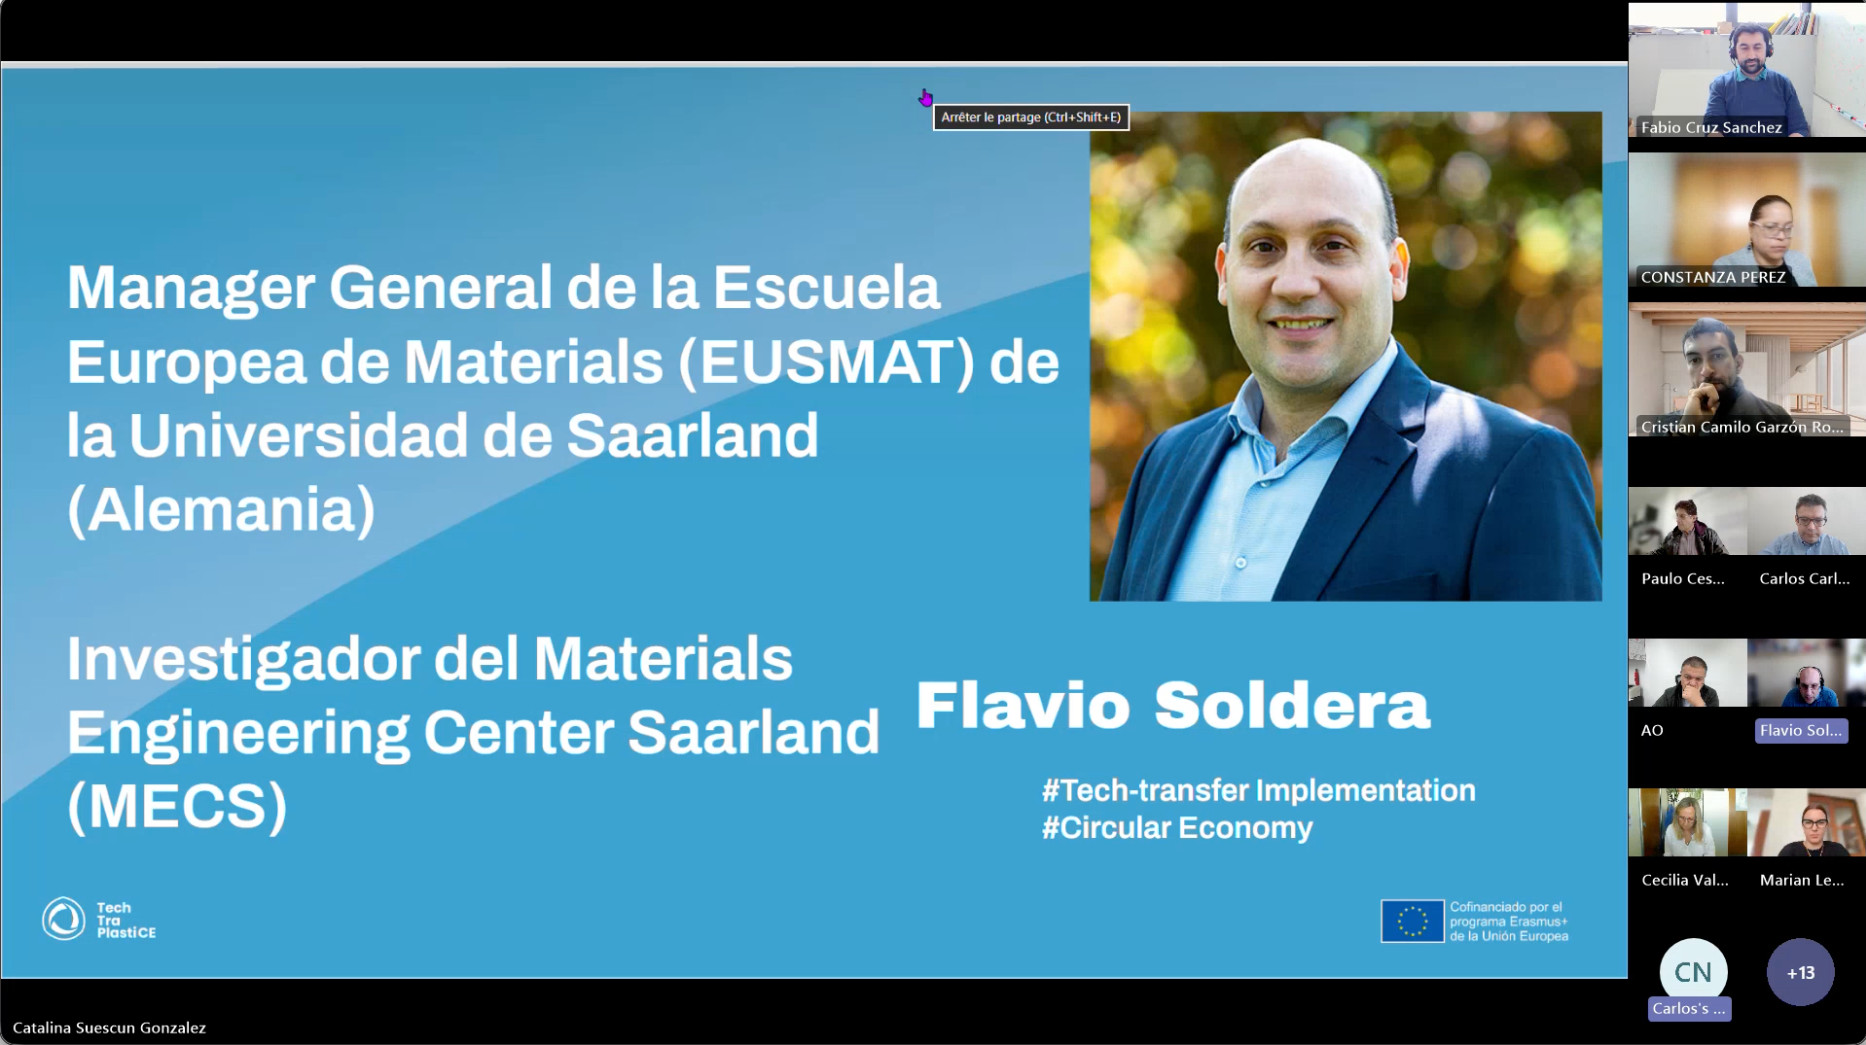
\includegraphics[keepaspectratio,alt={alt}]{figures/2.3/Flavio-00.jpg}}

}

\caption{\label{fig-flavio0}Presentation of Prof.~Flavio Soldera to the
TechTraPlastiCE Consortium on general meeting of April 2026}

\end{figure}%

\end{minipage}%
%
\begin{minipage}[t]{0.05\linewidth}
~\end{minipage}%
%
\begin{minipage}[t]{0.47\linewidth}

\begin{figure}[H]

\centering{

\pandocbounded{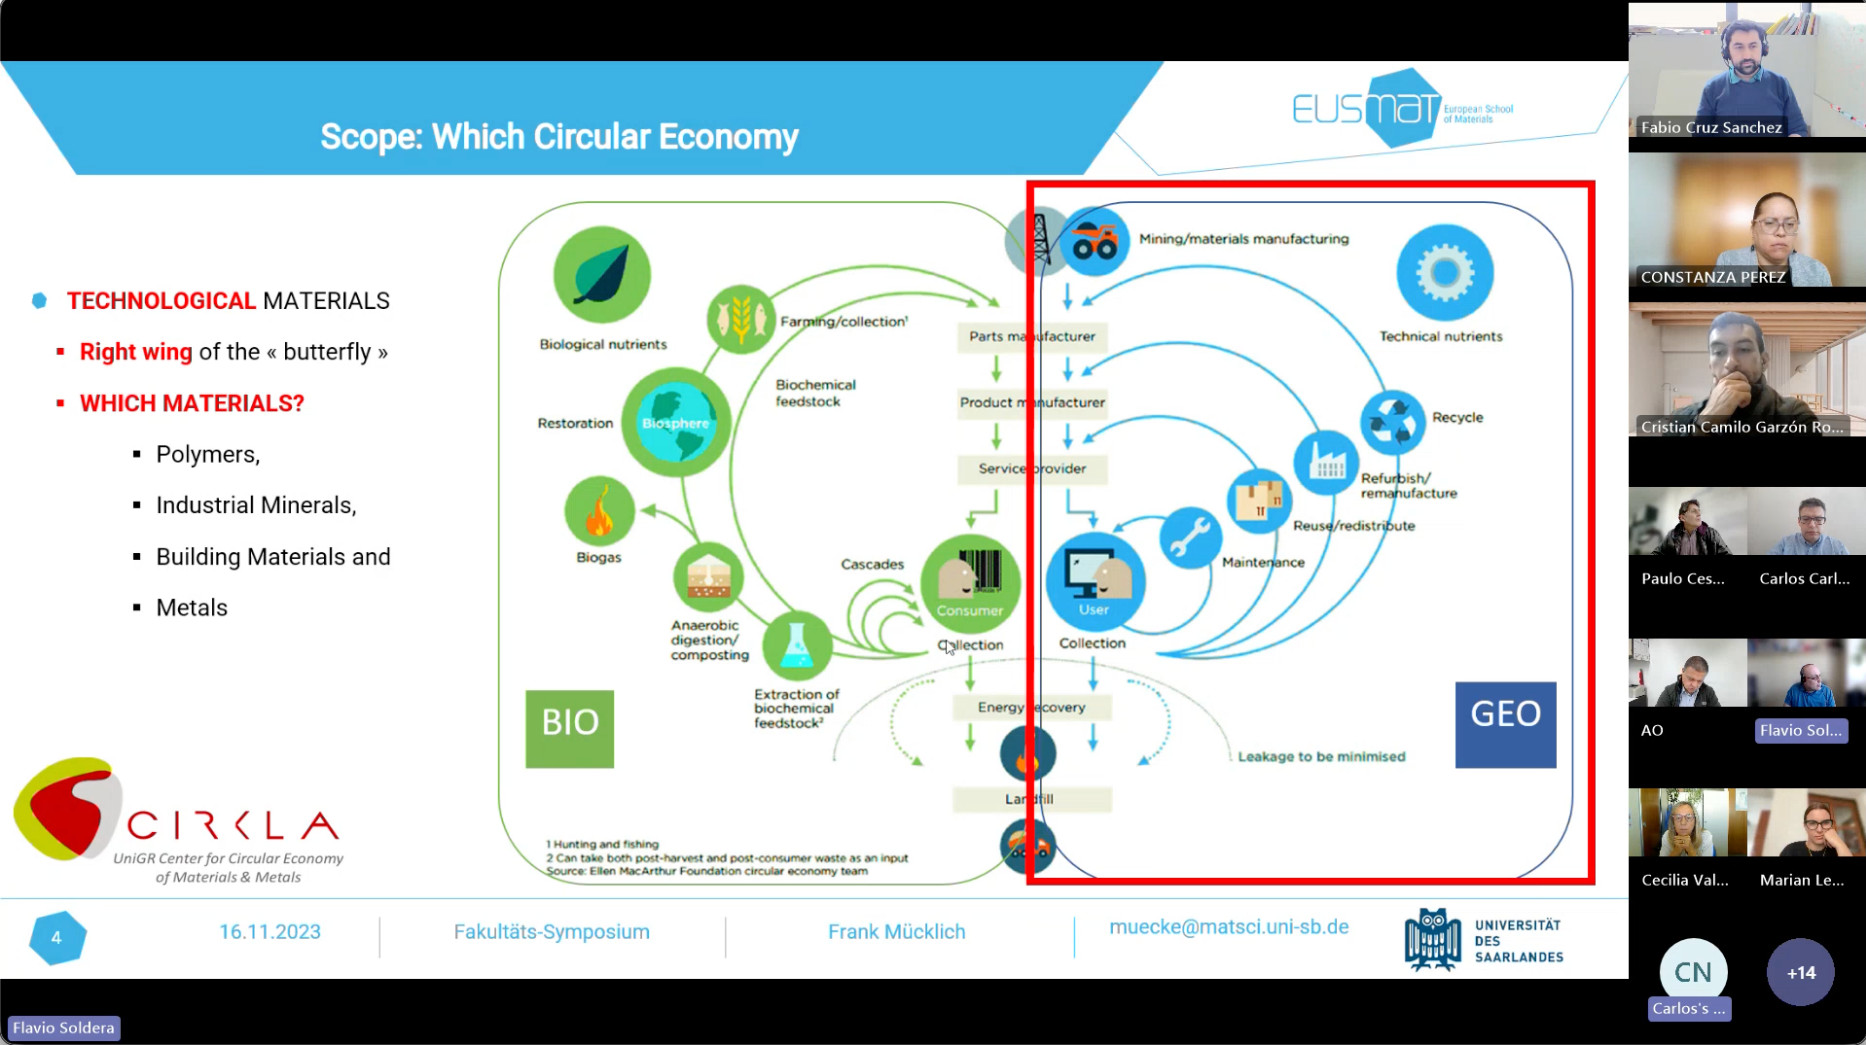
\includegraphics[keepaspectratio,alt={alt}]{figures/2.3/Flavio-01.jpg}}

}

\caption{\label{fig-flavio1}Prof.~Flavio Soldera presented the case of
CIRKLA project on circular economy}

\end{figure}%

\end{minipage}%

\end{figure}%

This interdisciplinary center of expertise, brings together numerous
activities around a clear mission: to create cross-border expertise
enabling more sustainable and balanced management of metals and
materials across all sectors of the economy and daily life. It is a
collective effort driven by shared awareness, practical experimentation,
and committed collaboration---at the crossroads of 4 countries, 3
languages, and numerous disciplines.

This cross-border initiative can be an example in the long term taht
could be applied to the latin american context.

\subsection{Marcos Maldonado -- Research and Development at the Ministry
of the Environment in
Chile.}\label{marcos-maldonado-research-and-development-at-the-ministry-of-the-environment-in-chile.}

Marcos Maldonado plays a key role in the design and coordination of
public policies related to science, technology, and innovation at Chile.
His expertise lies in innovation management, research coordination, and
the integration of scientific knowledge into policy and practice.

He holds dual Chilean and French degrees in Industrial and Systems
Engineering, as well as a Master II in Innovation Management and
Industrial Design. His professional experience includes the promotion
and management of innovation projects aligned with forestry and
agricultural priorities, contributing to sustainable development and the
articulation between scientific research and public policy.

\begin{figure}

\begin{minipage}[t]{0.47\linewidth}

\begin{figure}[H]

\centering{

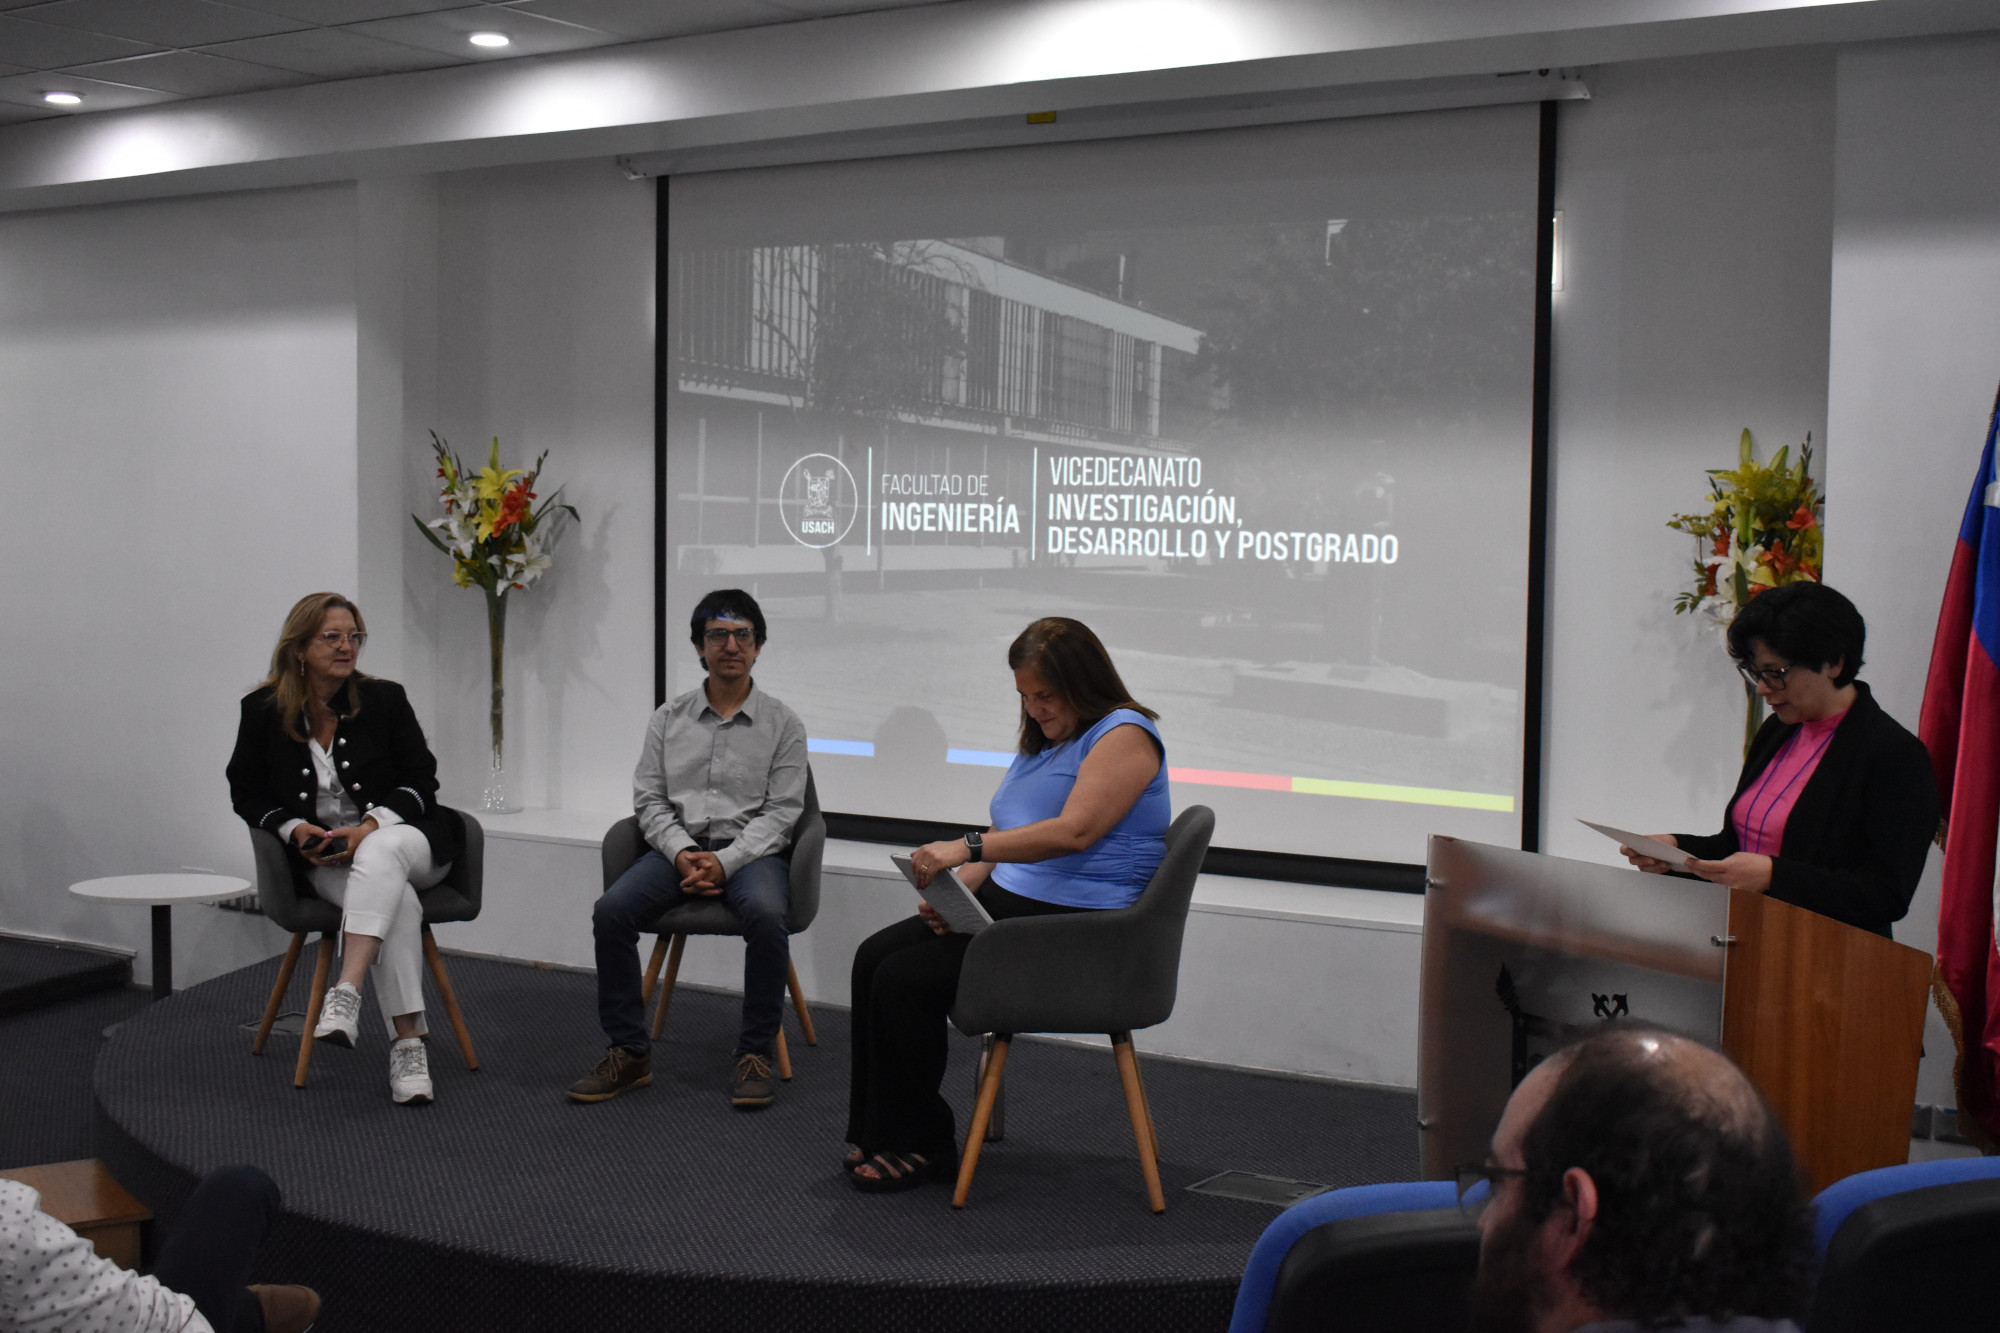
\includegraphics[width=0.9\linewidth,height=\textheight,keepaspectratio]{figures/2.3/Chile-00.jpg}

}

\caption{\label{fig-chile}Meeting of TechTraPlastiCE at Chile.
Nov.~2025}

\end{figure}%

\begin{figure}[H]

\centering{

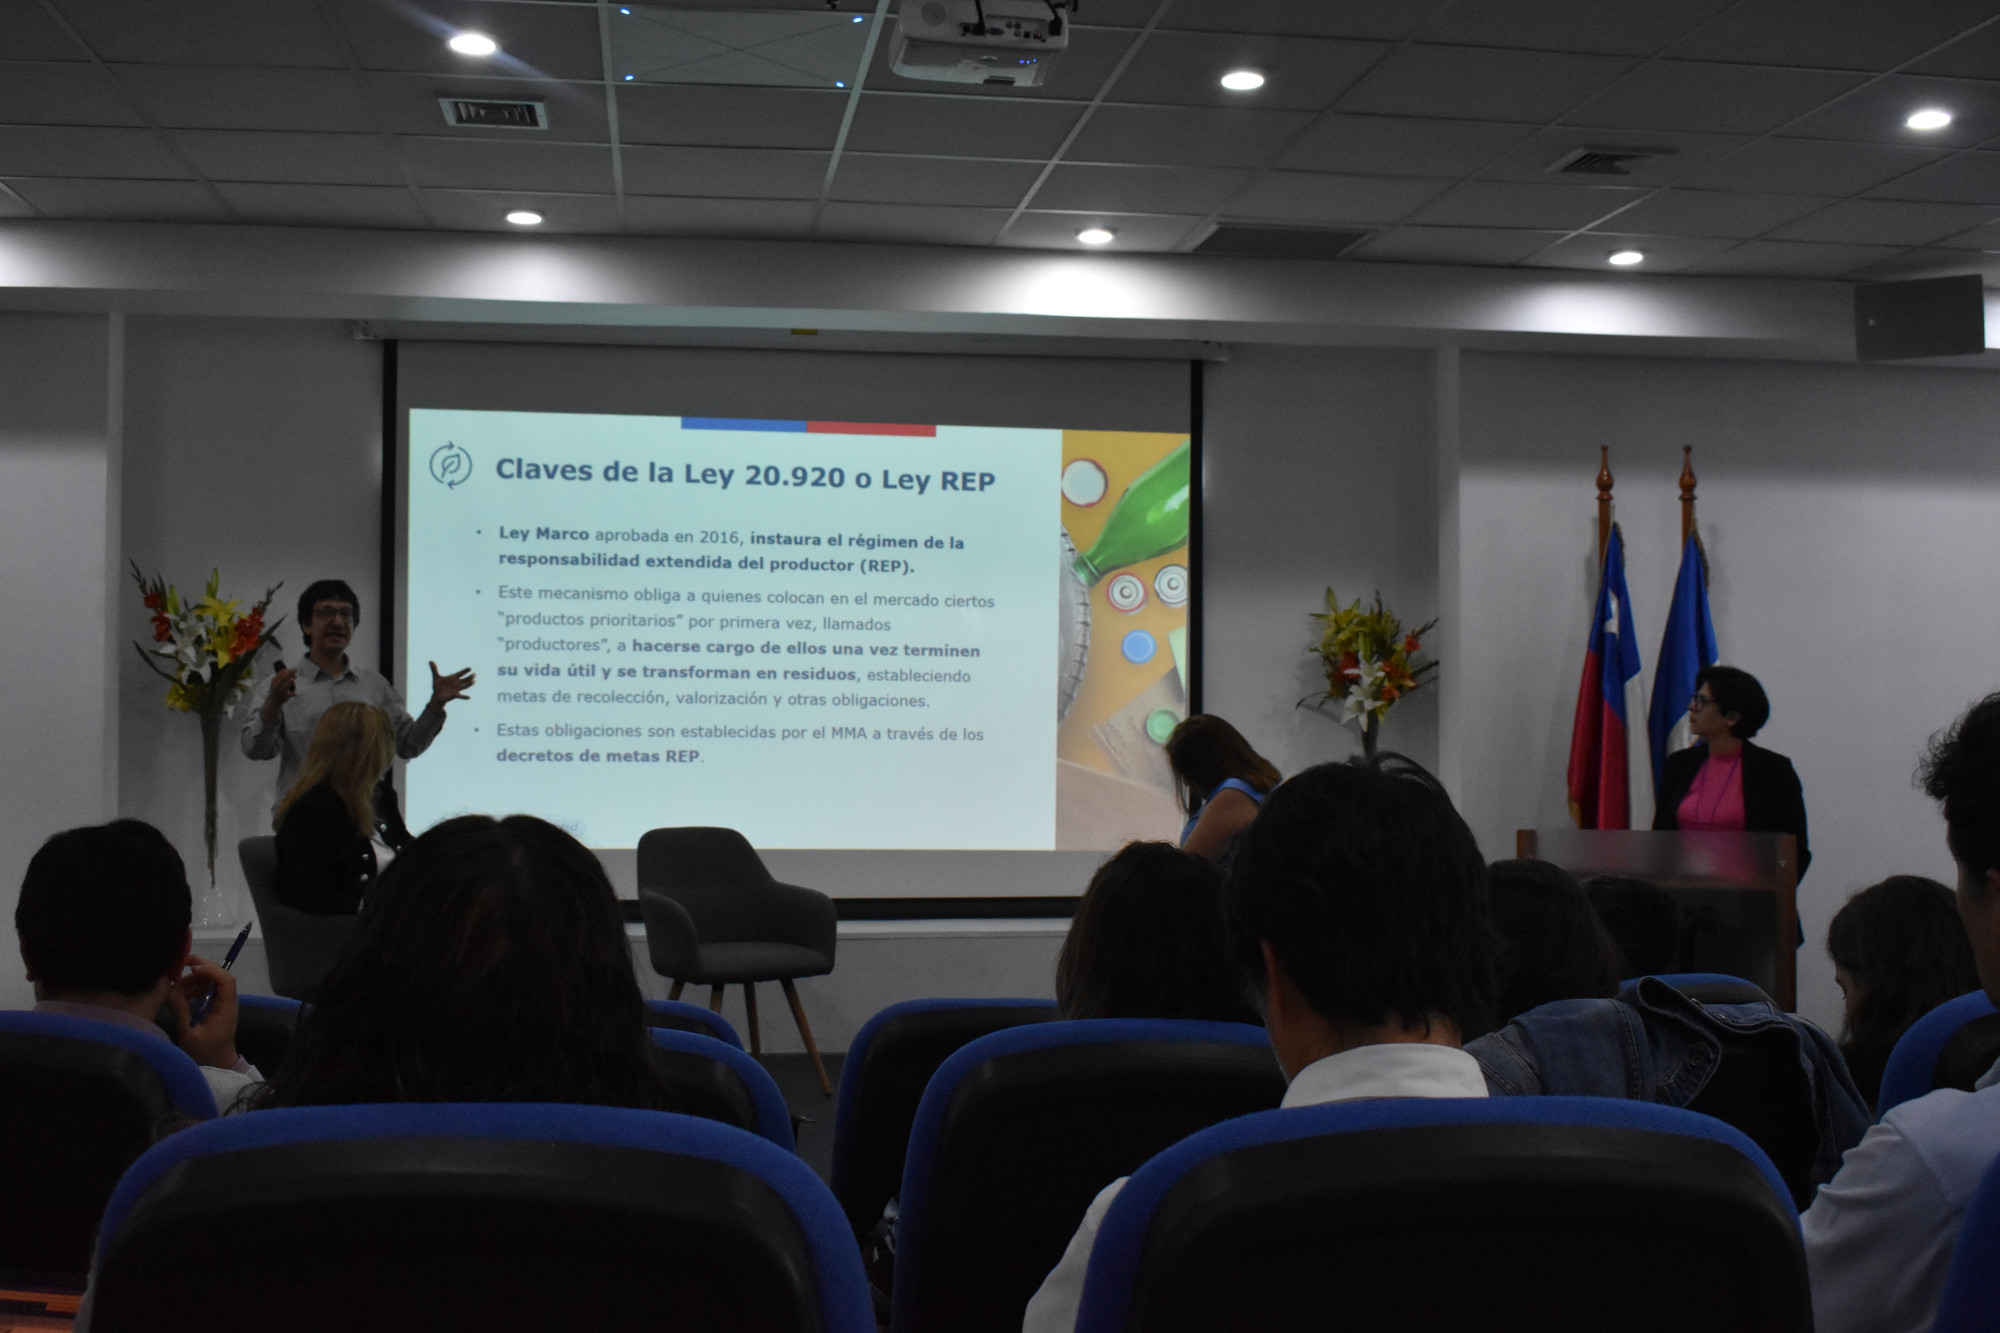
\includegraphics[width=0.9\linewidth,height=\textheight,keepaspectratio]{figures/2.3/Chile-01.jpg}

}

\caption{\label{fig-flavio1}Implementation of Extended Reponsability
scheme in Chile by Tomás Saieg}

\end{figure}%

\end{minipage}%
%
\begin{minipage}[t]{0.05\linewidth}
~\end{minipage}%
%
\begin{minipage}[t]{0.47\linewidth}

\begin{figure}[H]

\centering{

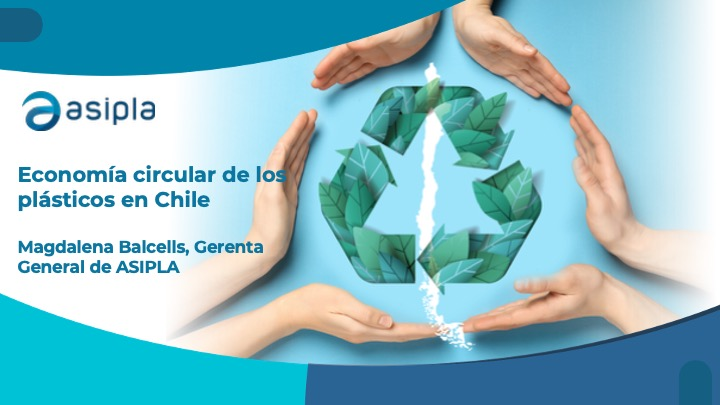
\includegraphics[width=0.9\linewidth,height=\textheight,keepaspectratio]{figures/2.3/Chile-02.jpg}

}

\caption{\label{fig-chile2}Presentation of Circular Economy of Plastics
In Chile by ASIPLA}

\end{figure}%

\begin{figure}[H]

\centering{

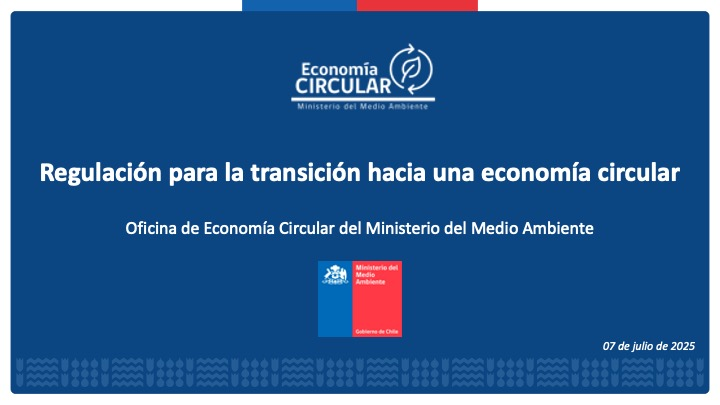
\includegraphics[width=0.9\linewidth,height=\textheight,keepaspectratio]{figures/2.3/Chile-03.jpg}

}

\caption{\label{fig-chile3}Towards Circular Economy by Ministery of
Environment}

\end{figure}%

\begin{figure}[H]

\centering{

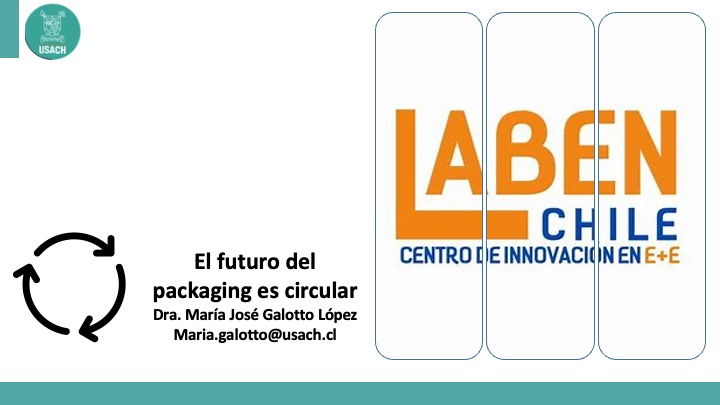
\includegraphics[width=0.9\linewidth,height=\textheight,keepaspectratio]{figures/2.3/Chile-04.jpg}

}

\caption{\label{fig-chile4}The future of Packaging is Circular by LABEN
(USACH Research Lab)}

\end{figure}%

\end{minipage}%

\end{figure}%

During the general meeting of TechTraPlastiCE in Chile, we had the
opportunity to introduce him to the consortium. Indeed, thanks to his
role at the Ministry of the Environment, it was possible to organize the
panel entitled: \emph{`Circular Economy in the Plastic Value Chain in
Chile: A shared challenge between government, academia and industry
within the framework of the TechTraPlastiCE project'} with Prof.~Andrea
Espinoza from USACH, Tomás Saieg (Office of Legislative Implementation
and Circular Economy of Chilean ministery) Magdalena Balcells -- ASIPLA
Asociación Gremial de Industriales del Plástico (Trade Association of
Plastics Manufacturers) and Prof.~María José Galotto (USACH) which leads
the ``Technology Center for Innovation in Packaging at the University of
Santiago, Chile (Centro Tecnológico de Innovación en Envases y Embalajes
Universidad de Santiago de Chile.
\href{https://www.labenchile.cl/}{LABEN CHILE-
https://www.labenchile.cl/})''.

This panel enlights the systemic problem of plastic and all perspectives
(goverment, industry and academia) that entails the transition towards
circular economy. The TechTraPlastiCE consortium had major interactions
and dicussions on the experience that Chilean context is taking place.
In the Annex Section~\ref{sec-planning}, the complete agenda of the
meeting can be found.

\newpage

\section{Identification of collaboration
opportunities}\label{identification-of-collaboration-opportunities}

The analysis of the canvas results revealed a strong shared recognition
of the value of collaborative work as a mechanism to enhance technology
transfer. Three main areas of collaboration were identified:

\begin{enumerate}
\def\labelenumi{\arabic{enumi}.}
\tightlist
\item
  \textbf{Integrated technological services}, including circularity
  assessment, eco-design, materials characterization, and validation of
  solutions in real environments.
\item
  \textbf{Joint applied R\&D projects}, focused on developing new
  materials, processes, and sustainable business models.
\item
  \textbf{Training and capacity-building initiatives}, such as joint
  programs, courses, workshops, and mobility schemes.
\end{enumerate}

In addition, more structural initiatives were proposed, including shared
technology transfer platforms, laboratory networks, and joint innovation
spaces, reflecting a move towards more institutionalized forms of
collaboration. From the perspective introduced through the open
innovation approach, these collaboration opportunities can also be
interpreted as potential co-creation processes, where institutions and
external stakeholders jointly define challenges and develop solutions
from early stages.

In this context, the analysis highlights the importance of moving beyond
traditional transfer mechanisms, such as service provision or technology
delivery, towards more interactive and iterative models of
collaboration. This includes the integration of interdisciplinary teams,
the use of participatory dynamics for problem definition, and the
progressive validation of solutions.

A relevant example discussed during this process was an applied case
developed at \emph{PLAPIQUI} \url{https://www.plapiqui.conicet.gov.ar/},
in which a challenge from the petrochemical sector was addressed through
a co-creation approach. The process involved the formation of
interdisciplinary teams, the generation of ideas through participatory
methodologies, and the systematic evaluation of alternatives based on
technical feasibility. This experience illustrates how open innovation
frameworks can support the transition from a broad set of initial ideas
to concrete solutions with transfer potential. These insights reinforce
the role of universities not only as providers of technological
solutions but also as strategic partners in collaborative innovation
processes.

\section{Workshop on cross-peer collaboration and mentoring
dynamics}\label{workshop-on-cross-peer-collaboration-and-mentoring-dynamics}

On March 26/2026, a virtual workshop was organized with the EAB Members
as presented in Figure~\ref{fig-eba}. We had the participation of 6 of
them.

\begin{figure}[H]

\centering{

\pandocbounded{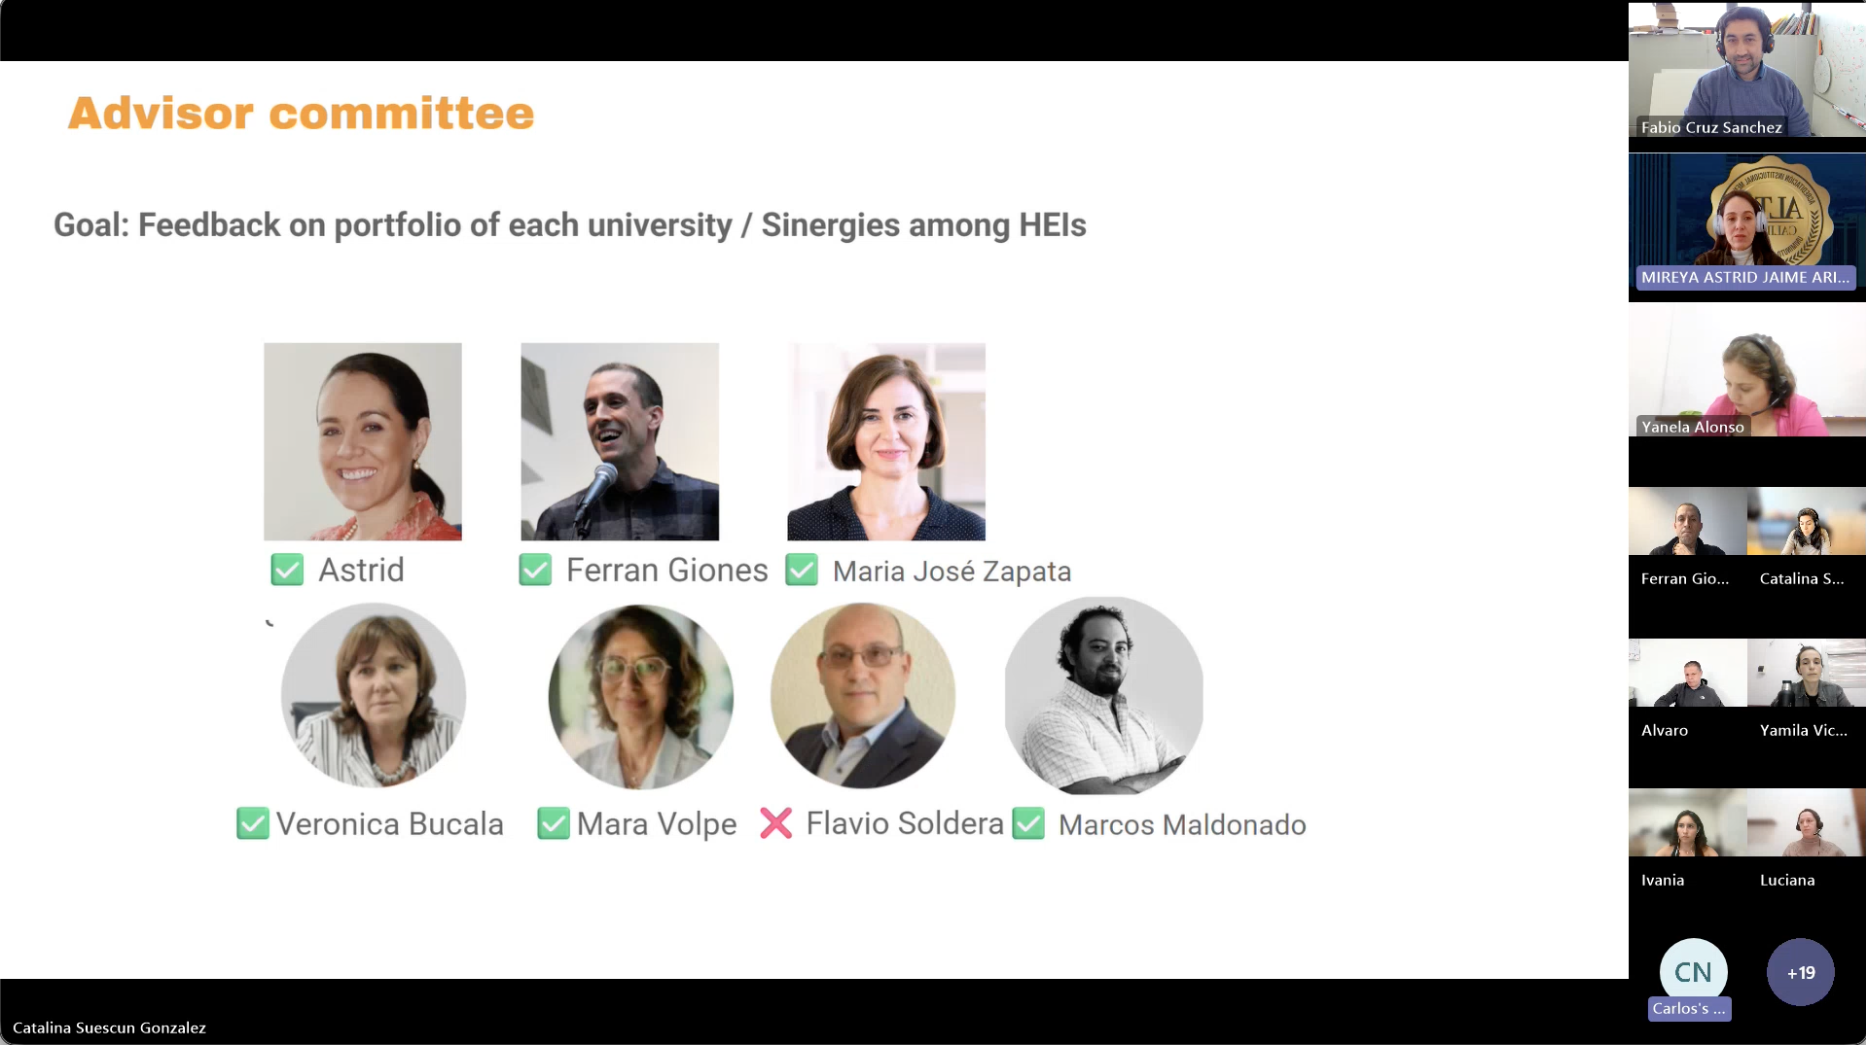
\includegraphics[keepaspectratio,alt={alt}]{figures/2.3/EBA.png}}

}

\caption{\label{fig-eba}Virtual workshop of the TechTraPlastiCE
Conssortium and external advisory board on March 26/2026.}

\end{figure}%

Tha major objective of the workshop was \emph{to foster the exchange of
experiences among Latin American universities from Chile, Colombia, and
Argentina, in order to deepen the understanding of the structural
opportunities and barriers identified in WP2, related to technology
transfer linked to the circular economy of the plastics value chain}.

The aim was to identify patterns, similarities, and differences in
approaches among universities, in order to obtain strategic
recommendations from members of the external advisory board to
strengthen both individual and collective service portfolios.

We structured the session in four blocks as follows:

\begin{enumerate}
\def\labelenumi{\arabic{enumi}.}
\tightlist
\item
  \textbf{Block 1 (10 min): Contextualization}

  \begin{itemize}
  \tightlist
  \item
    \textbf{TechTraPlastiCE Introduction (UL -- 3 min):} Introduction of
    the project's key objectives and clarification of the current stage
    of progress. The purpose of the session will also be explained,
    emphasizing that the goal is not to evaluate portfolios, but to
    understand how institutional contexts shape technology transfer.
  \item
    \textbf{Presentation of EBA Members (7 min total):} Introduction of
    the participating members of the External Advisory Board (EBA).
  \end{itemize}
\item
  \textbf{Block 2 (30 min): University Round (by regions: Argentina,
  Chile, Colombia, and Europe)}
\end{enumerate}

Each university will have \textbf{3 minutes} to highlight:

\begin{itemize}
\tightlist
\item
  Brief introduction of the speaker (profile, role within the
  university)
\item
  What should be the approach to tackling the challenge over the next 12
  months, including the methodology based on the conducted assessment
  and the specific institutional context
\item
  What concrete activities or actions they intend to implement, and what
  resources are available
\end{itemize}

For example, if the proposal is to strengthen institutional
coordination, the focus should now be on \textbf{how} they would act to
achieve this goal. This also helps refresh each university's context and
complements answers to the following questions:

\begin{itemize}
\tightlist
\item
  What was the most difficult aspect of mapping our portfolio?
\item
  What did we discover about our transfer culture?
\item
  What is currently our main institutional barrier?
\item
  If we had to prioritize a single critical point to improve within 12
  months, it would be.
\end{itemize}

\begin{enumerate}
\def\labelenumi{\arabic{enumi}.}
\setcounter{enumi}{2}
\tightlist
\item
  \textbf{Block 3 (30 min): Guided Discussion with Advisors}
\end{enumerate}

The questions for the advisors were around:

\begin{enumerate}
\def\labelenumi{\alph{enumi}.}
\tightlist
\item
  \textbf{Common Patterns}: Based on the videos and presentations:

  \begin{itemize}
  \tightlist
  \item
    What structural barriers are repeated across universities?
  \item
    What cultural or institutional patterns most influence technology
    transfer?
  \end{itemize}
\item
  \textbf{Differences Between Contexts}

  \begin{itemize}
  \tightlist
  \item
    What relevant differences do you identify among institutional or
    regional contexts?
  \item
    How do you think these differences affect transfer capacity?
  \end{itemize}
\item
  \textbf{Opportunities}

  \begin{itemize}
  \tightlist
  \item
    What strengths or opportunities do you see in the consortium that
    could be better leveraged collectively?
  \end{itemize}
\end{enumerate}

\begin{enumerate}
\def\labelenumi{\arabic{enumi}.}
\setcounter{enumi}{3}
\tightlist
\item
  \textbf{Block 4 (15 min): Final Strategic Recommendation}
\end{enumerate}

Final question to the EBA was :

\begin{itemize}
\tightlist
\item
  Based on what was observed across the consortium universities, what
  would be the \textbf{two strategic recommendations and/or
  intra/inter/extra-institutional synergies} that could help strengthen
  technology transfer in the short and medium term?
\end{itemize}

The results highlight the emergence of cross-peer collaboration and
mentoring opportunities within the consortium. Institutions identified
potential areas for knowledge exchange based on their relative
strengths, particularly in:

\begin{itemize}
\tightlist
\item
  Portfolio development and management,
\item
  Engagement with industry,
\item
  Implementation of transfer strategies and ,
\item
  Development of training and outreach activities.
\end{itemize}

This dynamic reflects the diversity of institutional profiles within the
consortium, where differences in experience, orientation, and maturity
create opportunities for mutual learning and support.

A distinction can be observed between institutions with more
consolidated transfer practices, which can act as mentors, and
institutions seeking to strengthen specific aspects of their transfer
systems. This complementary dynamic constitutes a key foundation for
structured peer-learning processes.

\subsection{Key barriers and strategic
recommendations}\label{key-barriers-and-strategic-recommendations}

The interaction with the EAB enabled the identification of common
barriers affecting technology transfer across institutions, including:

\begin{itemize}
\tightlist
\item
  Bureaucratic constraints and internal fragmentation,
\item
  Limited articulation with external stakeholders,
\item
  Low visibility of technological offerings,
\item
  Weak transfer culture and,
\item
  Lack of standardization.
\end{itemize}

In response, several strategic recommendations were highlighted:

\begin{itemize}
\tightlist
\item
  fostering internal coordination through formal and informal
  interaction spaces,
\item
  improving communication and visibility of institutional capacities,
\item
  adopting hybrid governance models,
\item
  implementing tools for managing interactions (e.g., Customer
  Relationship Management, CRM, systems),
\item
  and promoting long-term relationships with external stakeholders.
\end{itemize}

Additionally, technology transfer was emphasized as a continuous and
dynamic process, requiring ongoing portfolio updates and sustained
engagement with external actors.

\subsection{Towards a network-based transfer
model}\label{towards-a-network-based-transfer-model}

The results also demonstrated that the consortium has a strong potential
to evolve towards a more collaborative and network-based model of
technology transfer. The identification of complementarities, mentoring
opportunities, and shared challenges provides a solid foundation for
developing coordinated actions and joint initiatives.

At the same time, the results highlight the need to strengthen
coordination mechanisms, align institutional processes, and consolidate
communication channels. In this context, D2.3 represents a transition
from institutional capacity mapping to network activation, where
collaboration, peer-learning, and mentoring become key drivers for
enhancing the impact of technology transfer activities within the
plastic circular economy.

\section{Matching framework for cross-peer collaboration and
mentoring}\label{matching-framework-for-cross-peer-collaboration-and-mentoring}

Building upon the identification of institutional profiles (D2.2) and
the complementarities detected through the canvas analysis and the EAB
interaction, a structured matching framework was developed to facilitate
cross-peer collaboration and mentoring within the consortium. This
framework aims to connect partner institutions based on:

\begin{itemize}
\tightlist
\item
  their level of experience in technology transfer,
\item
  their dominant transfer profile (technical/technological, social,
  hybrid, etc.),
\item
  and their specific needs and strategic priorities.
\end{itemize}

Rather than a fixed pairing system, the matching approach is conceived
as a flexible and dynamic mechanism that enables different types of
collaboration depending on the context and objectives.

\subsection{Matching criteria}\label{matching-criteria}

Three main criteria were used to identify potential matches:

\begin{itemize}
\tightlist
\item
  \textbf{Affinity}: institutions sharing similar thematic interests
  (e.g., circular economy, materials, sustainability).
\item
  \textbf{Complementarity}: institutions with different but compatible
  capacities (e.g., advanced infrastructure vs.~territorial
  implementation).
\item
  \textbf{Mentoring potential}: institutions with more consolidated
  transfer practices supporting those seeking to strengthen specific
  capabilities.
\end{itemize}

\subsection{Types of matching
identified}\label{types-of-matching-identified}

Based on the analysis, three main types of matching were identified:

\begin{enumerate}
\def\labelenumi{\arabic{enumi}.}
\item
  \textbf{Mentoring-based matching: }focuses on knowledge transfer
  between institutions with different levels of experience.\\
  Examples:

  \begin{itemize}
  \tightlist
  \item
    Support in portfolio implementation
  \item
    Transfer of methodologies for engagement with industry
  \item
    Development of internal transfer structures
  \end{itemize}
\item
  \textbf{Complementarity-based matching: }combines different capacities
  to develop joint solutions or services.\\
  Examples:

  \begin{itemize}
  \tightlist
  \item
    Linking technological development with real-scale validation
  \item
    Integrating laboratory capabilities with territorial implementation
  \item
    Combining technical expertise with innovation management
  \end{itemize}
\item
  \textbf{Affinity-based matching:} connects institutions with similar
  orientations to scale activities or co-develop initiatives.\\
  Examples:

  \begin{itemize}
  \tightlist
  \item
    Joint training programs
  \item
    Collaborative research projects
  \item
    Shared thematic clusters
  \end{itemize}
\end{enumerate}

\subsection{Matching matrix and implementation
pathways}\label{matching-matrix-and-implementation-pathways}

Figure~\ref{fig-matchs} presents a proposed mapping of potential
interactions among partner institutions. Figure~\ref{fig-match0} propose
a mentoring-based match between the partners of the consortium.
Figure~\ref{fig-match1} propose a complementarity-based match while
Figure~\ref{fig-match2} present a affinity-based approach.

Table 1 describes potential actions between partners, with a focus on
specific activities. Both the figures and the table are classified
according to the type of matching. The process was not based on
arbitrary pairing, but on a systematic analysis of institutional
profiles, identifying how different types of capacities (technological,
managerial, and socio-territorial) can be articulated along the
technology transfer process.

\begin{figure}[H]

\begin{minipage}[t]{0.50\linewidth}

\centering{

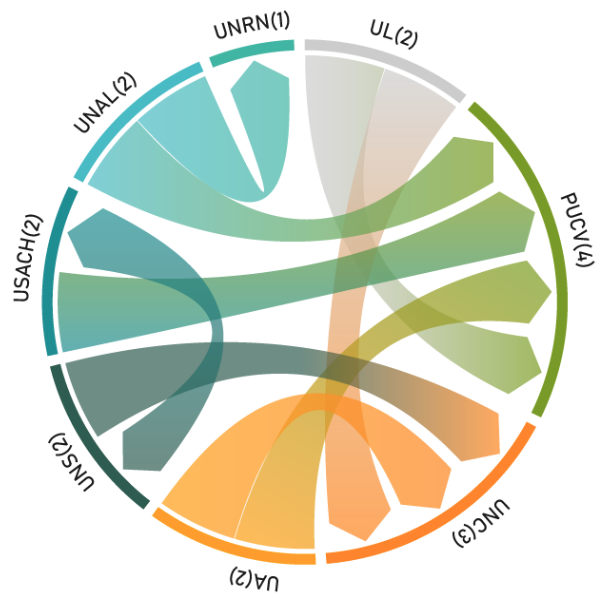
\includegraphics[width=3.125in,height=\textheight,keepaspectratio]{figures/2.3/Match-00.png}

}

\subcaption{\label{fig-match0}Mentoring-based matching}

\end{minipage}%
%
\begin{minipage}[t]{0.50\linewidth}

\centering{

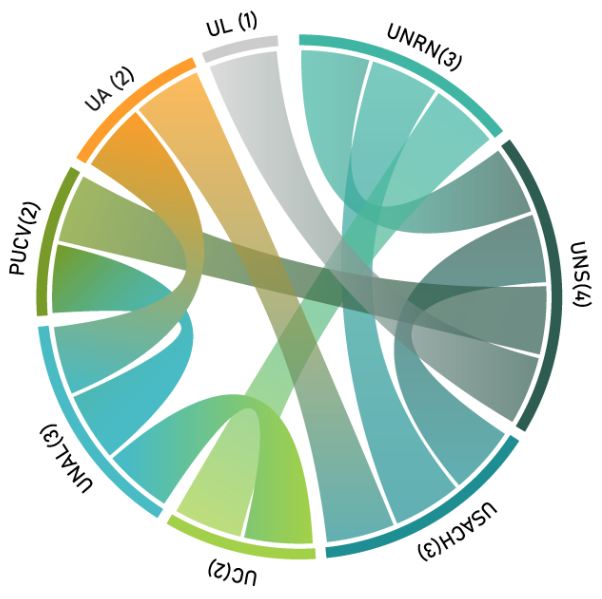
\includegraphics[width=3.125in,height=\textheight,keepaspectratio]{figures/2.3/Match-01.png}

}

\subcaption{\label{fig-match1}Complementarity-based matching}

\end{minipage}%
\newline
\begin{minipage}[t]{\linewidth}

\centering{

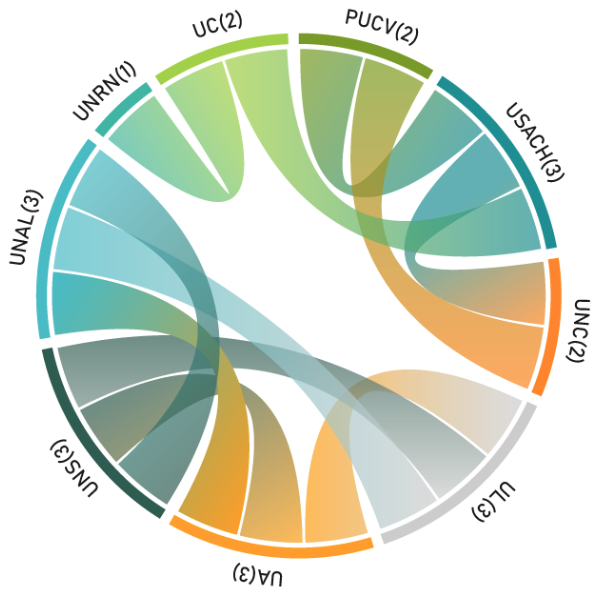
\includegraphics[width=3.125in,height=\textheight,keepaspectratio]{figures/2.3/Match-02.png}

}

\subcaption{\label{fig-match2}Affinity-based matching}

\end{minipage}%

\caption{\label{fig-matchs}Potential interactions among partner
institutions}

\end{figure}%

The matching matrix presented provides a structured representation of
potential collaboration pathways within the consortium, translating
institutional complementarities into concrete interaction opportunities.
Building on this analytical framework, the following section outlines
the operational mechanisms and actions required to activate these
matches and transform them into effective cross-peer collaboration and
mentoring dynamics.

\newpage

\begin{landscape}

\begingroup\fontsize{9}{11}\selectfont

\begin{longtable}[t]{>{\raggedright\arraybackslash}p{2.5cm}>{\raggedright\arraybackslash}p{3cm}>{\raggedright\arraybackslash}p{5cm}>{\raggedright\arraybackslash}p{3cm}>{\raggedright\arraybackslash}p{3cm}>{\raggedright\arraybackslash}p{3cm}}

\caption{\label{tbl-link}Matching matrix including the reason of the
potential links, their focus, the expected results and proposed
actions.}

\tabularnewline

\toprule
\begingroup\fontsize{12}{14}\selectfont \cellcolor{Naranja}{\textcolor{white}{\textbf{Type}}}\endgroup & \begingroup\fontsize{12}{14}\selectfont \cellcolor{Naranja}{\textcolor{white}{\textbf{Institutions}}}\endgroup & \begingroup\fontsize{12}{14}\selectfont \cellcolor{Naranja}{\textcolor{white}{\textbf{Justification (based on D2.2 profiles)}}}\endgroup & \begingroup\fontsize{12}{14}\selectfont \cellcolor{Naranja}{\textcolor{white}{\textbf{Focus}}}\endgroup & \begingroup\fontsize{12}{14}\selectfont \cellcolor{Naranja}{\textcolor{white}{\textbf{Expected outcome}}}\endgroup & \begingroup\fontsize{12}{14}\selectfont \cellcolor{Naranja}{\textcolor{white}{\textbf{Actions}}}\endgroup\\
\midrule
\endfirsthead
\multicolumn{6}{@{}l}{\textit{(continued)}}\\
\toprule
\begingroup\fontsize{12}{14}\selectfont \cellcolor{Naranja}{\textcolor{white}{\textbf{Type}}}\endgroup & \begingroup\fontsize{12}{14}\selectfont \cellcolor{Naranja}{\textcolor{white}{\textbf{Institutions}}}\endgroup & \begingroup\fontsize{12}{14}\selectfont \cellcolor{Naranja}{\textcolor{white}{\textbf{Justification (based on D2.2 profiles)}}}\endgroup & \begingroup\fontsize{12}{14}\selectfont \cellcolor{Naranja}{\textcolor{white}{\textbf{Focus}}}\endgroup & \begingroup\fontsize{12}{14}\selectfont \cellcolor{Naranja}{\textcolor{white}{\textbf{Expected outcome}}}\endgroup & \begingroup\fontsize{12}{14}\selectfont \cellcolor{Naranja}{\textcolor{white}{\textbf{Actions}}}\endgroup\\
\midrule
\endhead

\endfoot
\bottomrule
\endlastfoot
Complementarity & UNS -- USACH & UNS: strong technological development; USACH: innovation \& management tools & TRL scaling + innovation management & From prototype to implemented solution & Joint pilots, industry cases, co-designed services\\
\midrule\addlinespace
Complementarity & UNS -- UNRN & UNS: technological development; UNRN: territorial and socio-environmental implementation & Lab-to-territory transfer & Real-world validation of technologies & Field pilots, co-developed solutions with local actors\\
\midrule\addlinespace
Complementarity & UNAL -- UC & UNAL: advanced technical services; UC: socio-technical and policy-oriented approach & Integrated circular economy solutions & Combined technical, social, and policy impact & Joint consultancy, policy-oriented services\\
\midrule\addlinespace
Complementarity & UA -- USACH & UA: advanced infrastructure; USACH: innovation processes and management & Applied innovation processes & Increased readiness for industry application & Innovation labs, co-design workshops\\
\midrule\addlinespace
Complementarity & UL -- UNS & Both strong technical/technological profiles with advanced capabilities & Advanced materials \& processes & High-level technological solutions & Joint R\&D, shared infrastructure\\
\midrule\addlinespace
Complementarity & UA -- UNAL & UA: materials characterization; UNAL: bio-based developments & Material validation and scaling & Strengthened development pipeline & Testing protocols, joint validation\\
\midrule\addlinespace
Complementarity & PUCV -- UNS & PUCV: early-stage developments; UNS: scaling and engineering capacity & TRL progression & Scaling of technologies & Prototype-to-pilot transition projects\\
\midrule\addlinespace
Complementarity & USACH -- UNRN & USACH: innovation and management; UNRN: social and territorial implementation & Sustainable innovation systems & Context-adapted solutions & Territorial innovation pilots\\
\midrule\addlinespace
Complementarity & PUCV -- UNAL & PUCV: training \& early-stage innovation; UNAL: applied technological expertise & Knowledge-to-application integration & Stronger link between training and applied solutions & Joint training + applied pilot projects\\
\midrule\addlinespace
Complementarity & UC -- UNRN & Both with socio-territorial orientation but different approaches (policy vs implementation) & Social innovation in circular economy & Strengthened territorial impact strategies & Joint projects with local stakeholders\\
\midrule\addlinespace
Mentoring & UL, UA -- PUCV, UNC & EU: structured and consolidated services; LATAM: emerging structuring processes & Service standardization & More robust and structured portfolios & Templates, benchmarking, technical guidelines\\
\midrule\addlinespace
Mentoring & UNS -- UNC & UNS: consolidated technological profile; UNC: smaller scale and emerging structure & Strengthening technical transfer & Improved articulation between services and developments & Technical mentoring, lab practices\\
\midrule\addlinespace
Mentoring & USACH → PUCV & USACH: innovation-oriented; PUCV: hybrid profile & Innovation structuring & Stronger innovation component & Workshops, methodology transfer\\
\midrule\addlinespace
Mentoring (bidirectional) & UNS -- USACH & Complementarity between technological development and innovation management & Mutual learning & Integrated transfer models & Peer-learning exchanges, joint pilots\\
\midrule\addlinespace
Mentoring & UNAL -- PUCV, UNRN & UNAL: strong technical services and environmental focus & Strengthening applied services & Improved service portfolio quality & Training sessions, methodological transfer\\
\midrule\addlinespace
Affinity & PUCV, USACH, UNC & Hybrid profiles with strong training components & Training \& education & Expanded joint training offer & Joint courses, mobility programs\\
\midrule\addlinespace
Affinity & UL, UA, UNS, UNAL & Technical/technological profiles & Advanced services and R\&D & Consolidated technical offer & Shared service platforms, joint R\&D\\
\midrule\addlinespace
Affinity & UNRN, UC & Social and territorial orientation & Community engagement & Strengthened local impact & Joint territorial projects\\
\midrule\addlinespace
Affinity & USACH, UC & Strong orientation to management and innovation processes & Innovation and governance & Improved transfer strategies & Joint innovation frameworks\\
\midrule\addlinespace
Cross-cutting & All institutions & Shared need: visibility of capacities & Portfolio communication & Increased external engagement & Common platform, branding strategies\\
\midrule\addlinespace
Cross-cutting & All institutions & Weak articulation with industry (EAB insight) & Industry engagement & Stronger transfer impact & Demo days, brokerage events\\
\midrule\addlinespace
Cross-cutting & EU -- LATAM & Different maturity levels and institutional contexts & Knowledge transfer & Balanced capacity building & Staff exchange, mentoring schemes\\
\midrule\addlinespace
Cross-cutting & All institutions & Need for continuous transfer culture & Open innovation and co-creation & Dynamic collaboration ecosystem & Co-creation workshops, challenge-based collaboration, living labs\\
\midrule\addlinespace
Cross-cutting & All institutions & Need to systematize interactions and contacts & Transfer management & Improved traceability and efficiency & CRM systems, shared databases\\*

\end{longtable}

\endgroup{}

\end{landscape}

\subsection{Implementation/Operationalization of the matching
framework}\label{implementationoperationalization-of-the-matching-framework}

To ensure its practical implementation, the matching framework is
supported by a set of operational actions that could enable the
transition from identified opportunities to concrete collaboration
dynamics.

These actions include:

\begin{itemize}
\tightlist
\item
  \textbf{Peer-learning sessions} focused on specific challenges (e.g.,
  portfolio management, industry engagement).
\item
  \textbf{Mentoring schemes}, where more experienced institutions
  support others through structured exchanges.
\item
  \textbf{Joint pilot initiatives}, allowing the testing of
  collaborative services or solutions.
\item
  \textbf{Co-development of training activities}, including courses,
  workshops, and mobility programs.
\item
  \textbf{Collaborative project development}, aimed at leveraging
  complementarities for future funding opportunities.
\end{itemize}

This operational perspective proposal ensures that the matching process
is not limited to analytical identification but evolves into actionable
collaboration pathways, aiming to reinforce the long-term impact of the
consortium.

\subsection{Illustrative cases of cross-peer collaboration and
mentoring}\label{illustrative-cases-of-cross-peer-collaboration-and-mentoring}

As part of the bidirectional mentoring dynamic identified between UNS
and USACH, based on the complementarity between technological
development capacities and innovation management approaches, several
concrete collaboration initiatives have begun to emerge, illustrating
the operationalization of the matching framework.

A first relevant experience is linked to the implementation of the
\emph{``48 hours of innovation'' activity planned within the
TechTraPlastiCE project at UNS during the second half of 2026}. In this
context, USACH has provided methodological support and training to UNS
for the design and execution of this initiative, transferring practical
knowledge on innovation dynamics, facilitation strategies, and
impact-oriented approaches. This exchange not only reflects a mentoring
process but also a co-learning dynamic, where methodologies are adapted
to the local institutional context.

\textbf{Building on this interaction, a new elective course on
innovation has been introduced within the Chemical Engineering
Department at UNS}. The course design has been directly informed by the
experience and guidance provided by USACH, incorporating approaches
aimed at strengthening students' innovation capabilities and also,
preparing them for active participation in the ``48 hours of
innovation'' initiative. This represents a concrete example of how
knowledge transfer between institutions can be embedded into academic
structures, amplifying its impact through education and capacity
building.

In parallel, institutional-level interactions have been initiated
between the internationalization offices of UNS and USACH, aiming to
explore and consolidate longer-term collaboration mechanisms. Within the
existing framework of the Asociación de Universidades Grupo Montevideo
(AUGM), discussions have led to the proposal of implementing the
innovation course as a ``mirror course'' (cátedra espejo) in both
institutions. This initiative would enable synchronized teaching
experiences, fostering shared learning environments and setting a
precedent for future joint academic activities. Additionally,
preliminary discussions have explored the potential development of joint
postgraduate or specialization programs, although these initiatives
require further institutional alignment and regulatory processes.

Beyond the UNS--USACH collaboration, additional inter-institutional
linkages have been identified within the consortium. In particular,
emerging interactions between UNS (including PLAPIQUI) and the
Universidad Nacional de Córdoba (UNC) are being strengthened through the
connection with the Instituto de Procesos y Química Aplicada (IPQA).
This institute, currently established within UNC as a research and
development unit, originated from scientific and technological
capacities initially developed at PLAPIQUI (UNS--CONICET), later
evolving towards institutional independence. This shared trajectory
provides a strong foundation for collaboration, as it reflects not only
complementary capacities but also a common scientific background and
aligned research approaches. In this context, with the collaboration of
thehhte Secretariat of Sustainable Policies, exchanges between
researchers involved in sustainability-related lines within the project,
the Faculty of Dentistry and IPQA members have enabled the
identification of potential joint initiatives focused on plastics
sustainability. These prospective collaborations aim to articulate
advanced research capabilities with applied technology transfer,
reinforcing long-term cooperation between both institutions.

Furthermore, synergies have been identified with other Erasmus+ Capacity
Building projects within UNS, particularly the EduSAF project
(\url{https://www.edusafproject.eu/}). Although focused on the agri-food
sector, EduSAF shares a strong emphasis on innovation, capacity
building, and university--society interaction. Initial exchanges between
both projects have opened opportunities for cross-project collaboration,
especially in areas related to innovation methodologies, training
approaches, and stakeholder engagement strategies. This highlights the
potential for scaling impact not only within the TechTraPlastiCE
consortium but also across parallel Erasmus+ initiatives.

Overall, these experiences illustrate how the identified matching
dynamics can evolve into concrete actions, combining mentoring,
co-development, and institutional collaboration. They also demonstrate
that cross-peer interaction extends beyond bilateral exchanges, enabling
the creation of broader innovation ecosystems that integrate multiple
institutions and projects.

\chapter{Conclusions}\label{conclusions}

This deliverable consolidates the transition from the identification and
structuring of institutional capacities (D2.2) to their activation
through collaboration and peer-learning processes within the consortium.

Results demonstrated that the diversity of institutional profiles
constitutes a key asset, enabling the development of complementary and
synergistic interactions among partners. The identification of
collaboration opportunities, combined with the emergence of mentoring
dynamics, provides a strong foundation for advancing towards more
coordinated and effective technology transfer practices.

Moreover, the perspective of the External Advisory Board contributed
with valuable strategic insights, reinforcing the need to address
structural barriers while adopting a long-term and dynamic approach to
technology transfer.

In this context, D2.3 highlights the importance of moving towards a
network-based model, where collaboration, knowledge exchange, and mutual
support enhance the capacity of higher education institutions to respond
to the challenges of the plastic circular economy and to generate impact
at regional and international levels.

\chapter{Annex}\label{annex}

\section{Agenda of the Presential Consortium Meeting in Santiago de
Chile.}\label{sec-planning}

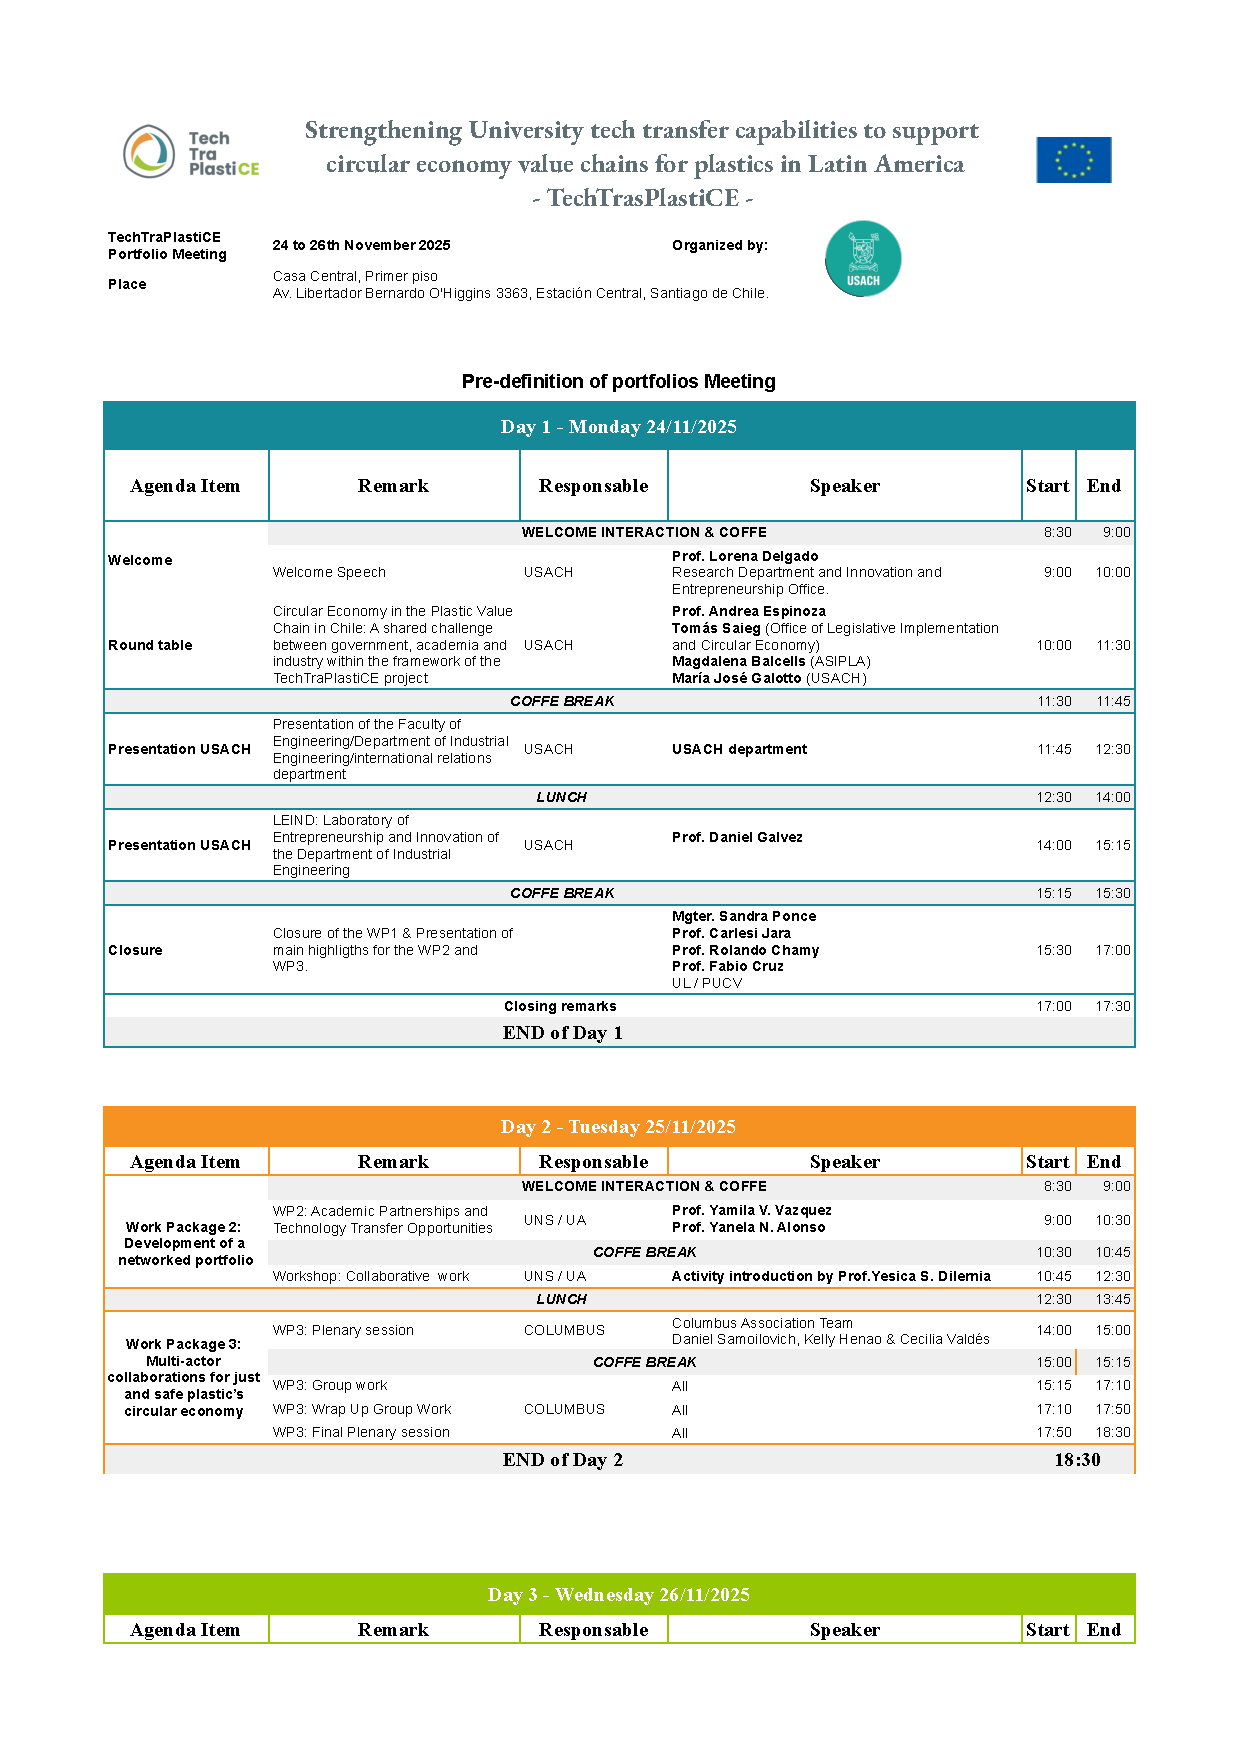
\includepdf[pagecommand={\pagestyle{fancy}}, scale=0.9,
pages=-]{figures/2.3/Agenda.pdf}

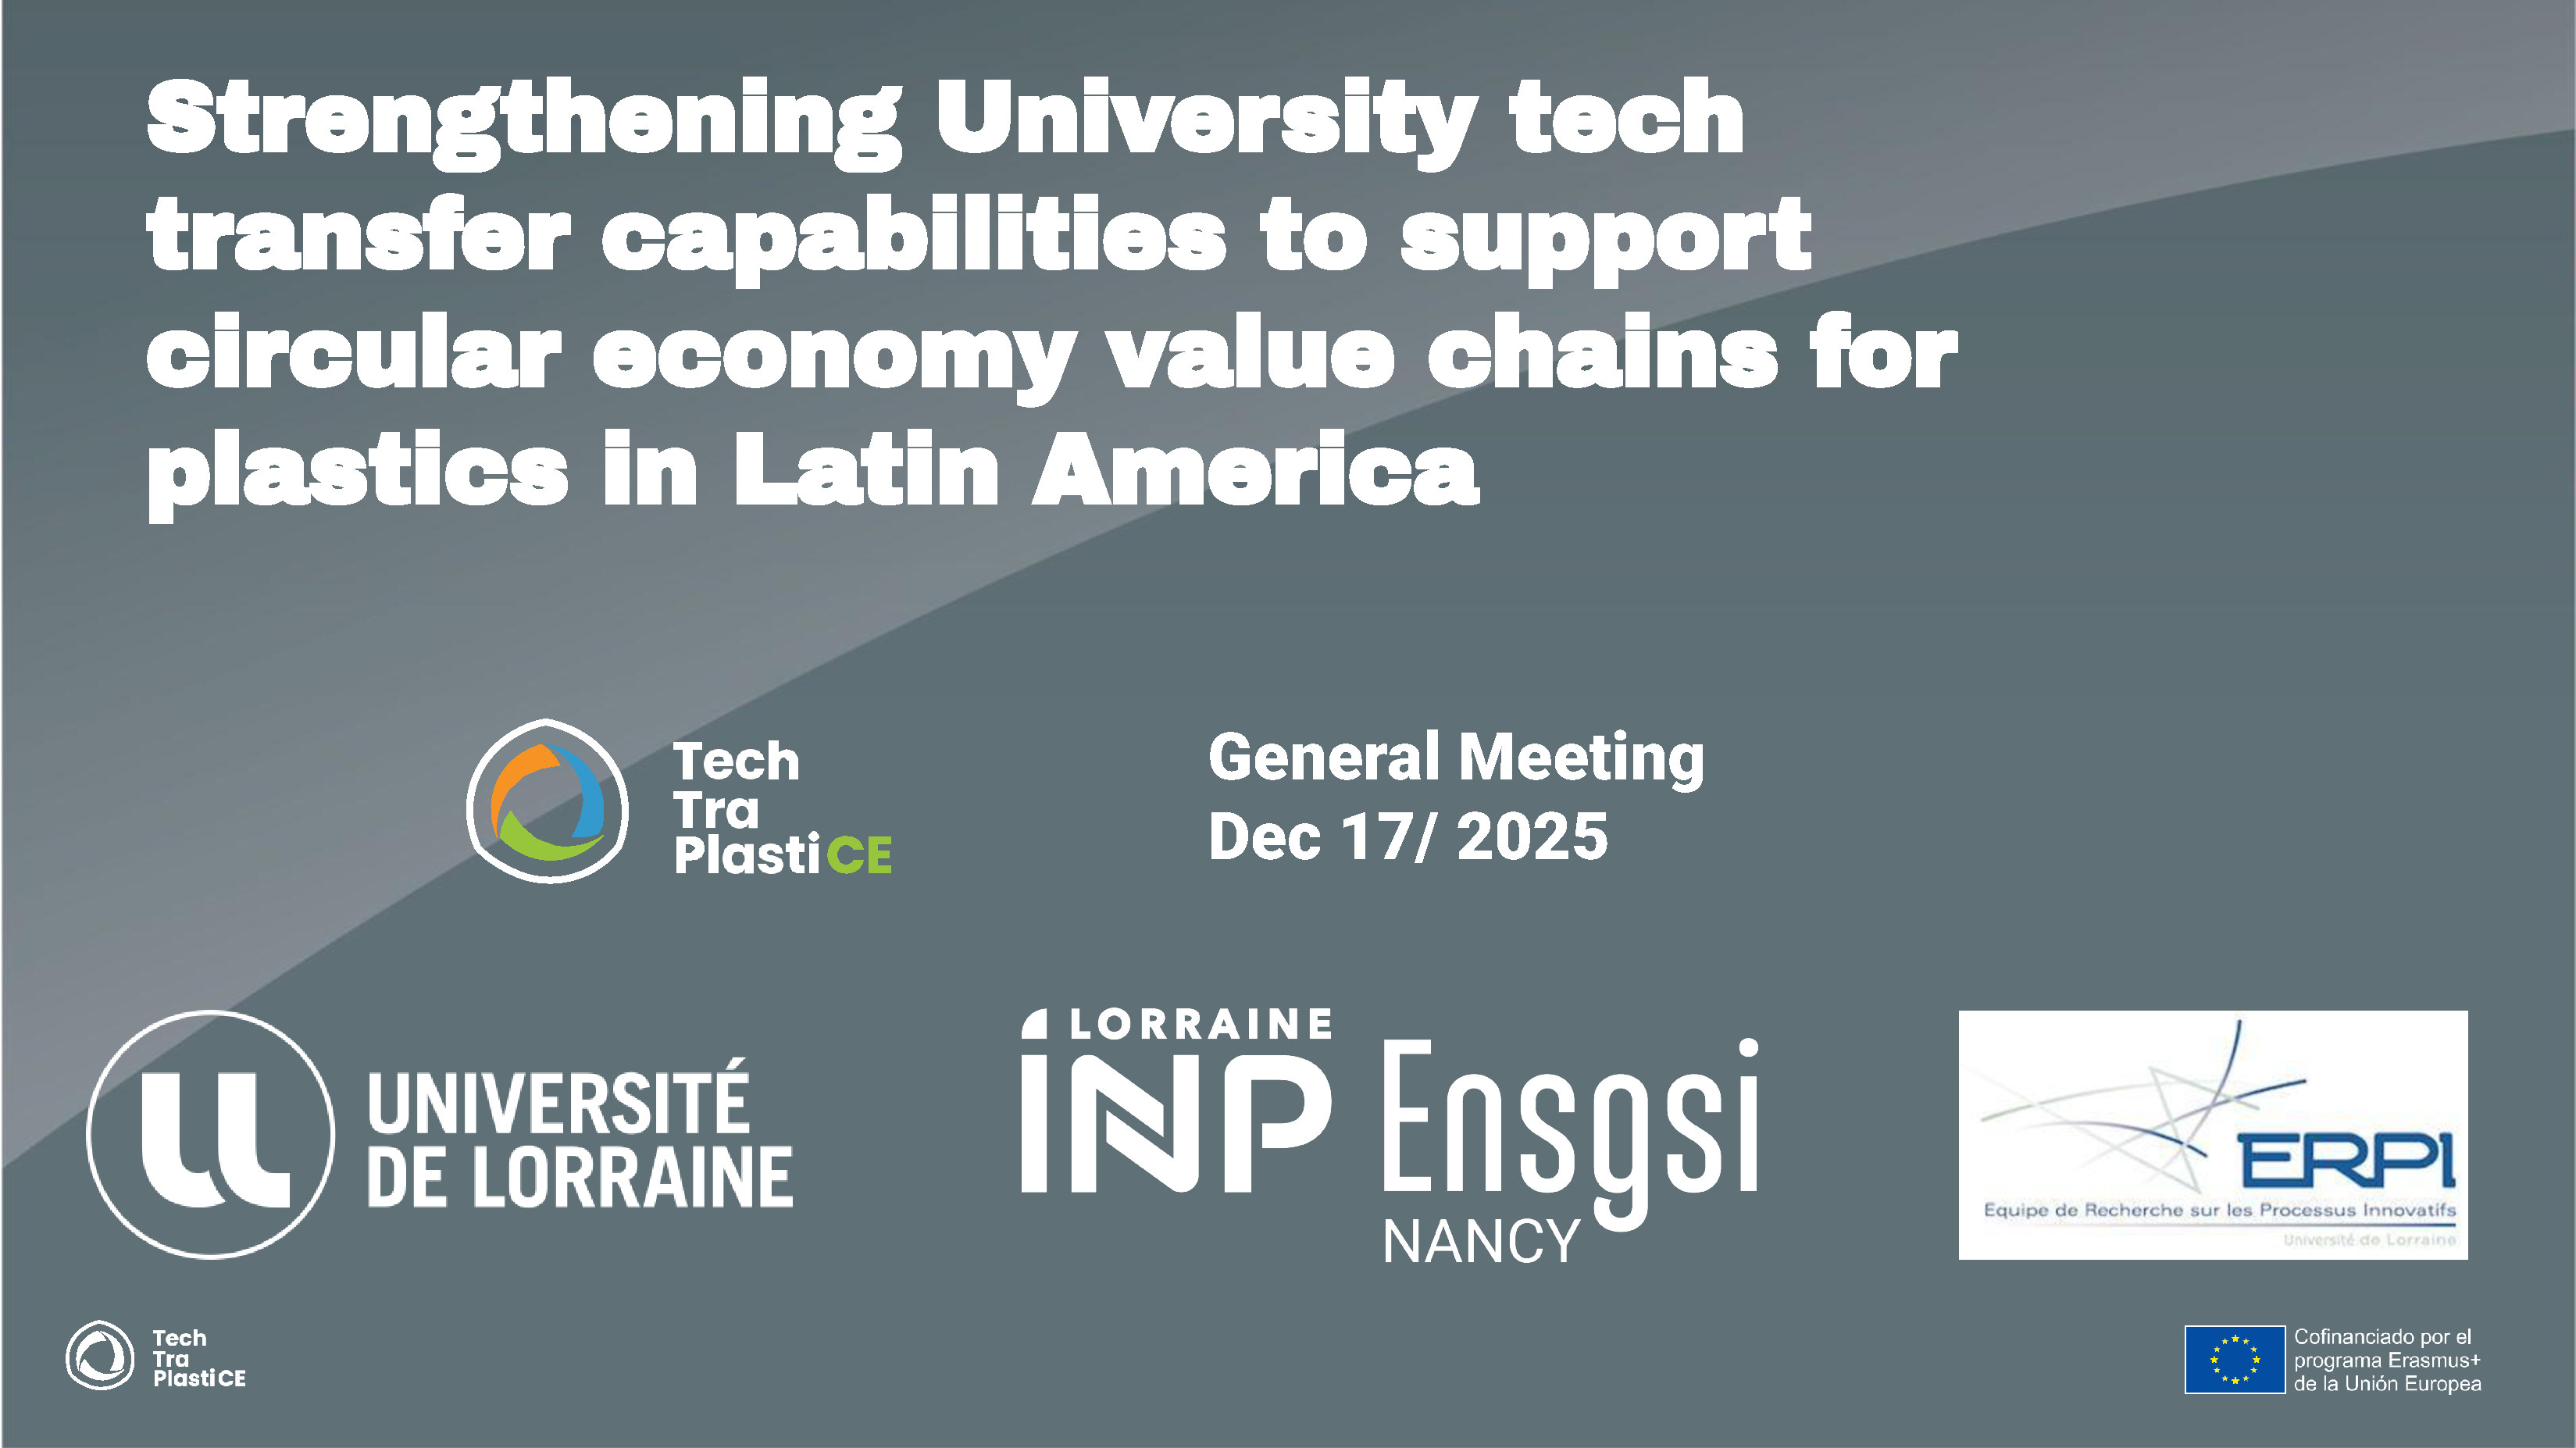
\includepdf[landscape=false,  delta=2 2, frame=true,  nup=2x3, pagecommand*={\pagestyle{fancy} \section{Presentation of Open Innovation and presentation of Véronica Bucala and Mara Volpe on General Meeting of Dec. 17/2025}}, 
scale=0.8, pages=-]{annex/2.3/2025-12-17-General-Meeting.pdf}


\backmatter


\end{document}
